\documentclass[12pt]{article}

\usepackage{
    amssymb,
    amsmath,
    amsfonts,
    eurosym,
    geometry,
    ulem,
    graphicx,
    caption,
    color,
    setspace,
    sectsty,
    comment,
    footmisc,
    caption,
    natbib,
    pdflscape,
    subfigure,
    array,
    hyperref,
    booktabs,
    longtable,
    float,
    threeparttable}
% \usepackage[
%     backend=biber,
%     style=nature,
%     doi=false,
%     isbn=false,
%     url=false,
%     eprint=false
%     ]{biblatex}
        

\normalem

\onehalfspacing
\newtheorem{theorem}{Theorem}
\newtheorem{corollary}[theorem]{Corollary}
\newtheorem{proposition}{Proposition}
\newenvironment{proof}[1][Proof]{\noindent\textbf{#1.} }{\ \rule{0.5em}{0.5em}}

\newtheorem{hyp}{Hypothesis}
\newtheorem{subhyp}{Hypothesis}[hyp]
\renewcommand{\thesubhyp}{\thehyp\alph{subhyp}}

\newcommand{\red}[1]{{\color{red} #1}}
\newcommand{\blue}[1]{{\color{blue} #1}}

\newcolumntype{L}[1]{>{\raggedright\let\newline\\arraybackslash\hspace{0pt}}m{#1}}
\newcolumntype{C}[1]{>{\centering\let\newline\\arraybackslash\hspace{0pt}}m{#1}}
\newcolumntype{R}[1]{>{\raggedleft\let\newline\\arraybackslash\hspace{0pt}}m{#1}}

\geometry{left=1.0in,right=1.0in,top=1.0in,bottom=1.0in}

\addbibresource{lipids.bib}

\begin{document}

\begin{titlepage}
\title{Long-term and recent trends in serum cholesterol awareness, treatment, and control in 12 high-income countries: an analysis of 90 nationally representative surveys\thanks{abc}}
\author{NCD Risk Factor Collaboration (NCD-RisC) 
    \thanks{Christopher B. Boyer (Harvard TH Chan School of Public Health, Boston, MA, USA); Bin Zhou (Imperial College London, London, UK); Goodarz Danaei (Harvard TH Chan School of Public Health, Boston, MA, USA); Majid Ezzati (Imperial College London, London, UK); \ldots}}
\date{\today}
\maketitle
\begin{abstract}
\noindent Placeholder\\
\vspace{0in}\\
\noindent\textbf{Keywords:} key1, key2, key3\\

\bigskip
\end{abstract}
\setcounter{page}{0}
\thispagestyle{empty}
\end{titlepage}
\pagebreak \newpage

    


\doublespacing


\section{Introduction} \label{sec:introduction}

\section{Methods} \label{sec:methods}

\section{Results} \label{sec:result}

\section{Discussion} \label{sec:discussion}

%\section{Conclusion} \label{sec:conclusion}



\singlespacing



\clearpage

\onehalfspacing

\section*{Tables} \label{sec:tab}
\addcontentsline{toc}{section}{Tables}

\begin{table}[H]
    \centering
    \begin{tabular}[t]{lccc}
    \toprule
    & Non-HDL-C & Eligible & Treated\\
    \midrule
    woman & \num{-0.040} & \num{-0.145}*** & \num{0.043}*\\
     & (\num{0.037}) & (\num{0.021}) & (\num{0.018})\\
    age50-59 years & \num{0.255}*** & \num{0.182}*** & \num{0.071}***\\
     & (\num{0.021}) & (\num{0.020}) & (\num{0.008})\\
    age60-69 years & \num{0.244}*** & \num{0.405}*** & \num{0.090}***\\
     & (\num{0.038}) & (\num{0.031}) & (\num{0.015})\\
    age70-79 years & \num{0.131}* & \num{0.634}*** & \num{0.037}\\
     & (\num{0.051}) & (\num{0.028}) & (\num{0.029})\\
    woman × post2010 & \num{-0.418}*** & \num{0.018} & \num{0.126}***\\
     & (\num{0.043}) & (\num{0.015}) & (\num{0.017})\\
    age50-59 years × post2010 & \num{-0.345}*** & \num{-0.019} & \num{0.034}+\\
     & (\num{0.029}) & (\num{0.013}) & (\num{0.016})\\
    age60-69 years × post2010 & \num{-0.620}*** & \num{-0.119}*** & \num{0.125}**\\
     & (\num{0.049}) & (\num{0.015}) & (\num{0.035})\\
    age70-79 years × post2010 & \num{-0.765}*** & \num{-0.171}*** & \num{0.127}*\\
     & (\num{0.068}) & (\num{0.018}) & (\num{0.042})\\
    woman × age50-59 years × post2010 & \num{0.480}*** & \num{-0.002} & \num{-0.017}\\
     & (\num{0.023}) & (\num{0.018}) & (\num{0.031})\\
    woman × age60-69 years × post2010 & \num{0.692}*** & \num{0.059}+ & \num{-0.094}**\\
     & (\num{0.063}) & (\num{0.030}) & (\num{0.023})\\
    woman × age70-79 years × post2010 & \num{0.779}*** & \num{0.142}*** & \num{-0.190}***\\
     & (\num{0.049}) & (\num{0.027}) & (\num{0.019})\\
    \midrule
    Observations & \num{314368} & \num{255369} & \num{107879}\\
    $R^2$ Adj. & \num{0.074} & \num{0.237} & \num{0.192}\\
    % Std.Errors & by: iso \& mid\_year & by: iso \& mid\_year & by: iso \& mid\_year\\
    FE: Country & Yes & Yes & Yes\\
    FE: Year & Yes & Yes & Yes\\
    \bottomrule
    \multicolumn{4}{l}{\rule{0pt}{1em}+ p $<$ 0.1, * p $<$ 0.05, ** p $<$ 0.01, *** p $<$ 0.001}\\
\end{tabular}
\end{table}

\clearpage

\section*{Figures} \label{sec:fig}
\addcontentsline{toc}{section}{Figures}

\begin{figure}[hp]
 \centering
 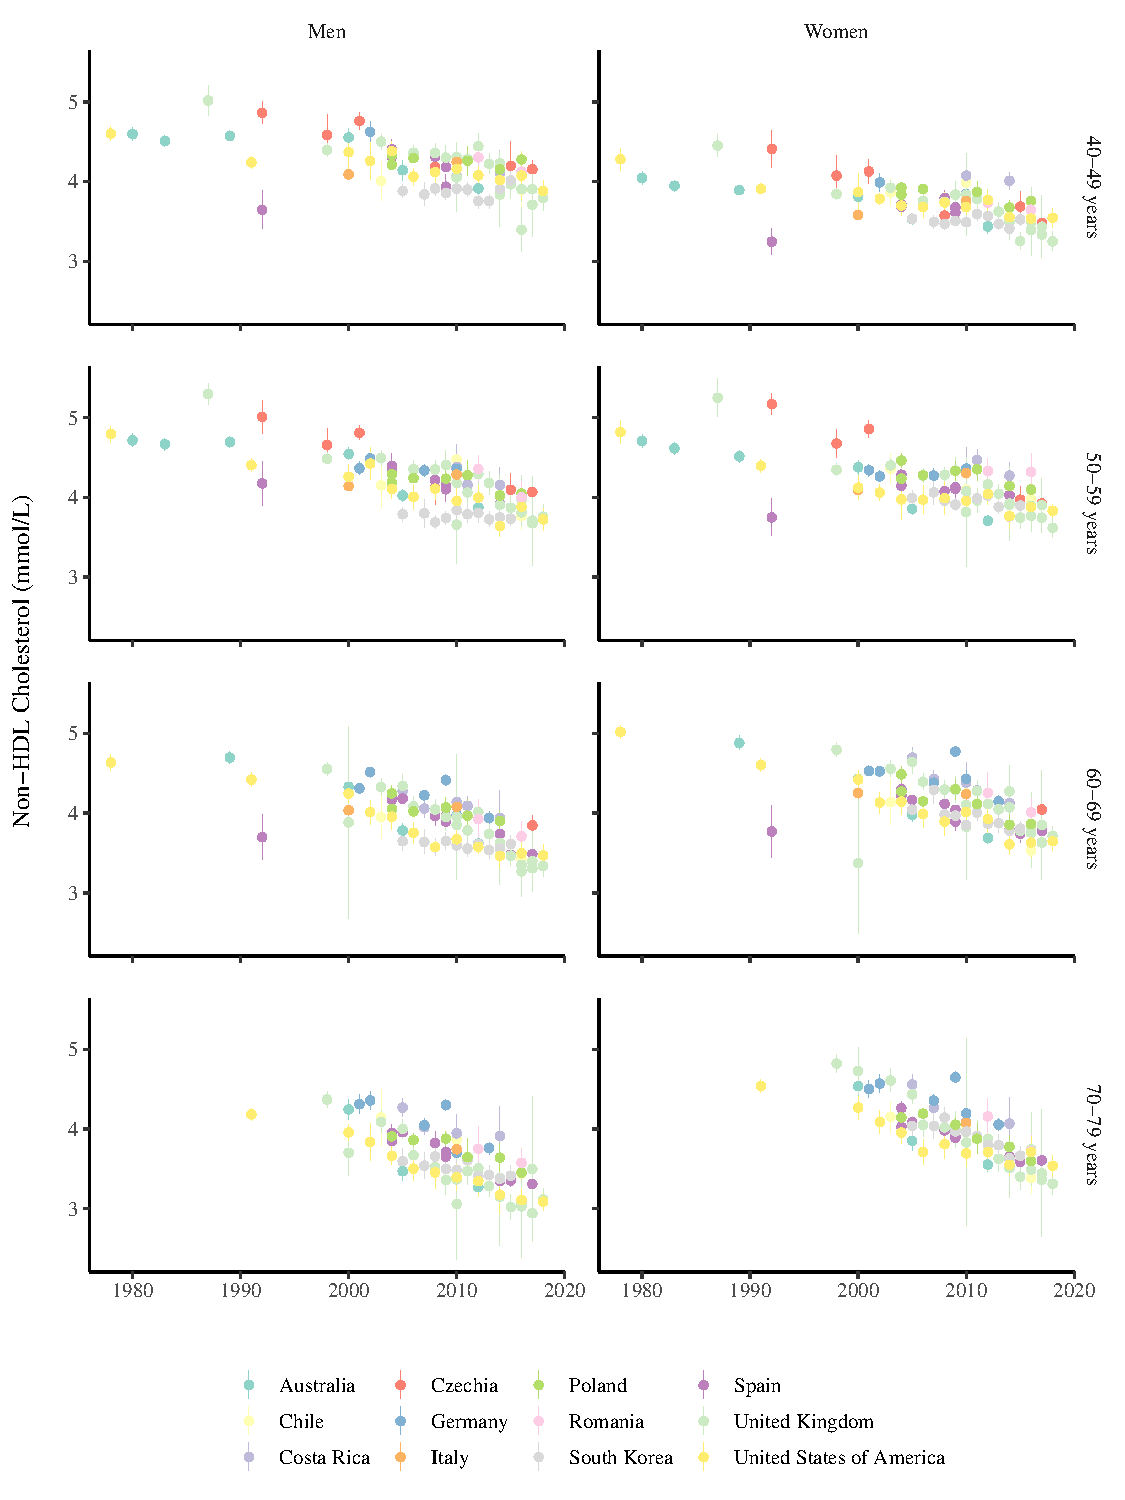
\includegraphics[width=\textwidth]{../3_figures/fig1_mean_chol.pdf}
 \caption{Trends in mean non-HDL serum cholesterol level, by country, sex, and age group.}
 \label{fig:mean_chol}
\end{figure}

\begin{figure}[hp]
    \centering
    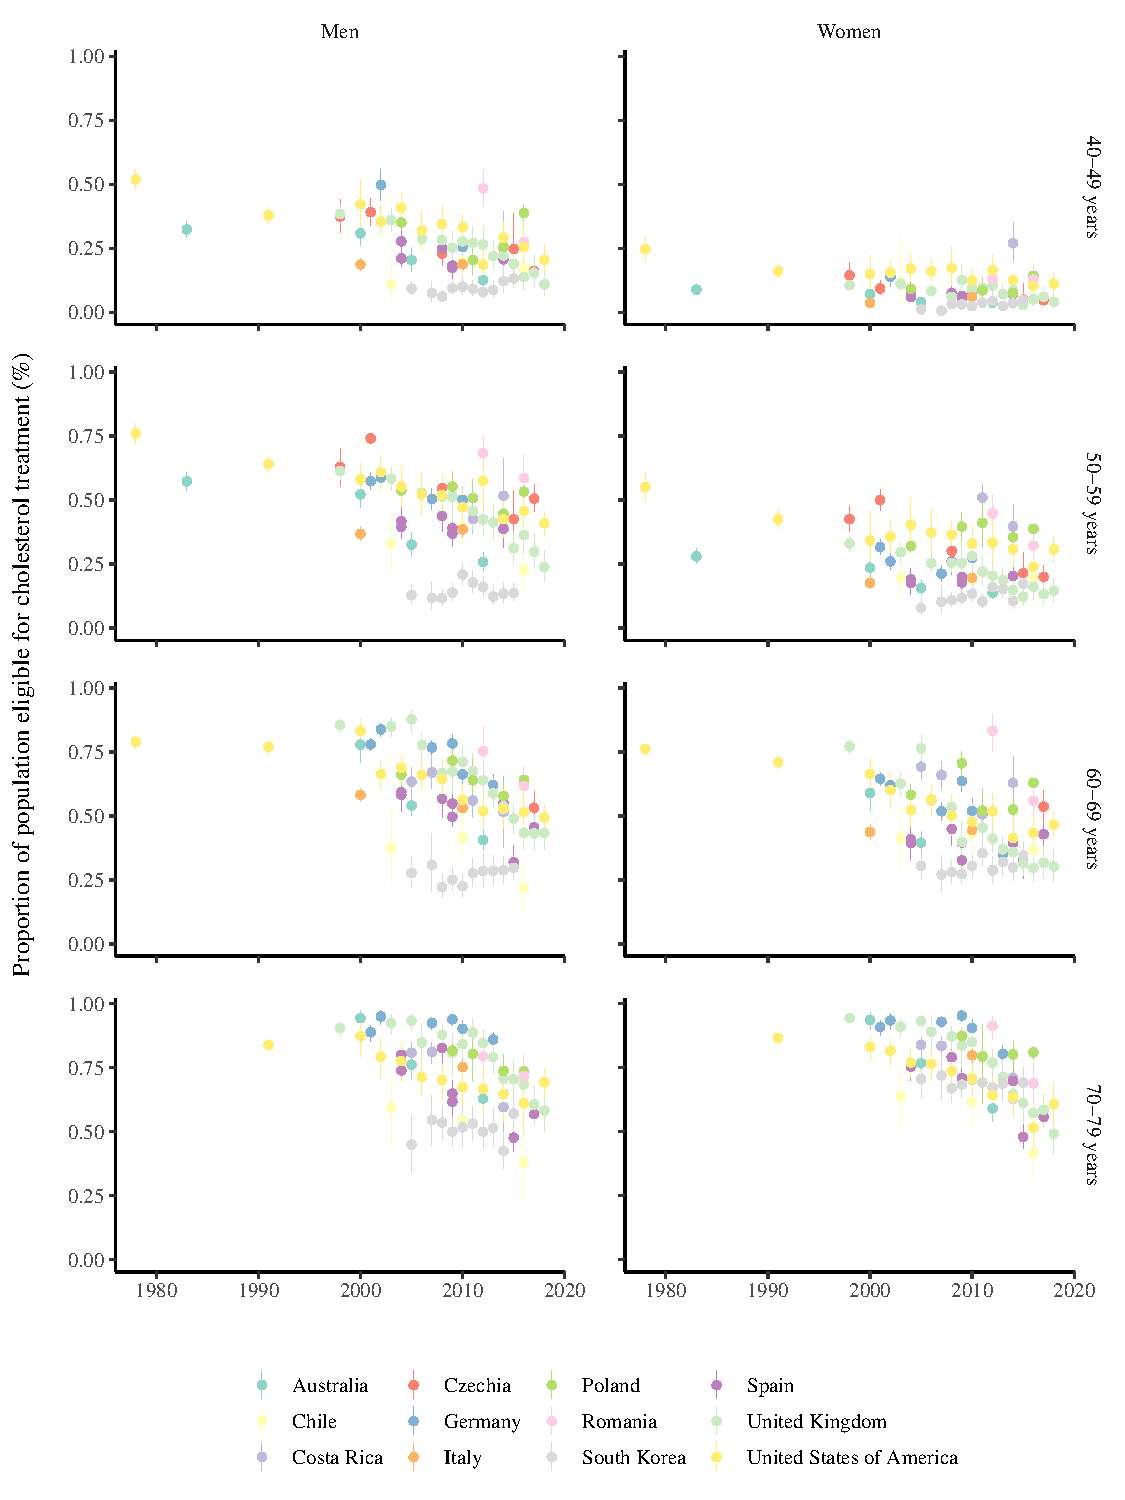
\includegraphics[width=\textwidth]{../3_figures/fig2_eligible.pdf}
    \caption{Trends in eligibility for cholesterol treatment, by country, sex, and age group.}
    \label{fig:eligible}
\end{figure}

\begin{figure}[hp]
    \centering
    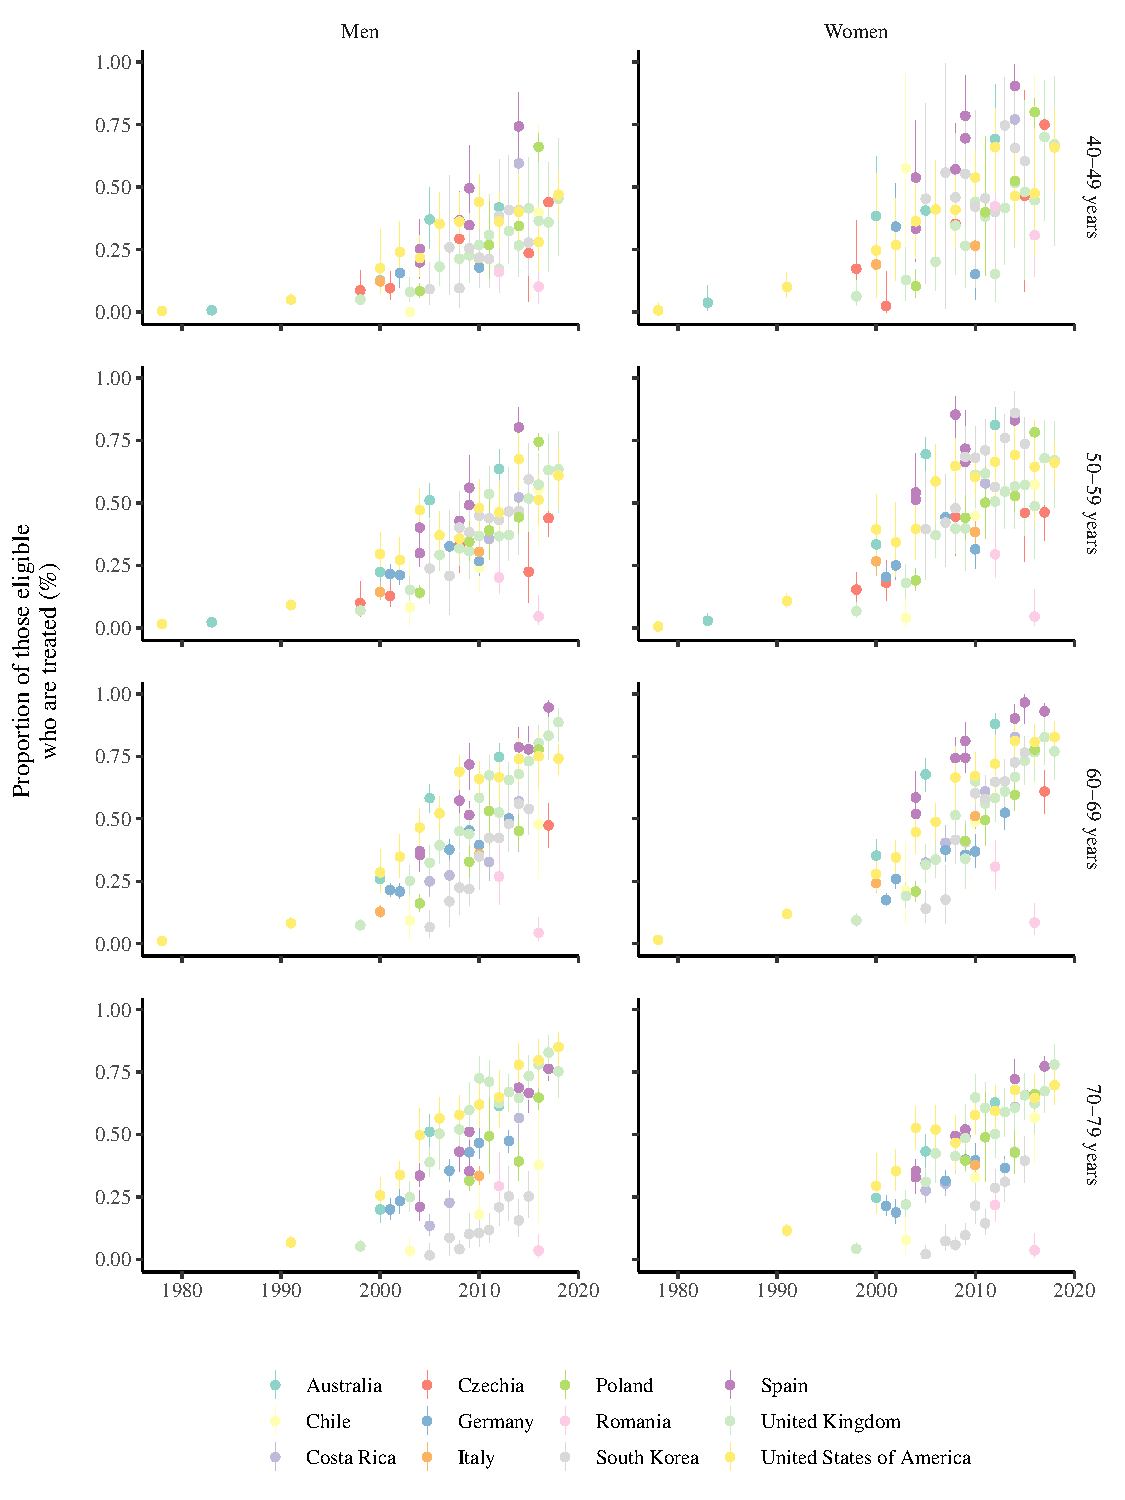
\includegraphics[width=\textwidth]{../3_figures/fig3_treated.pdf}
    \caption{Trends in cholesterol treatment among people with elevated serum cholesterol, by country, sex, and age group.}
    \label{fig:treated}
\end{figure}

\begin{figure}[hp]
    \centering
    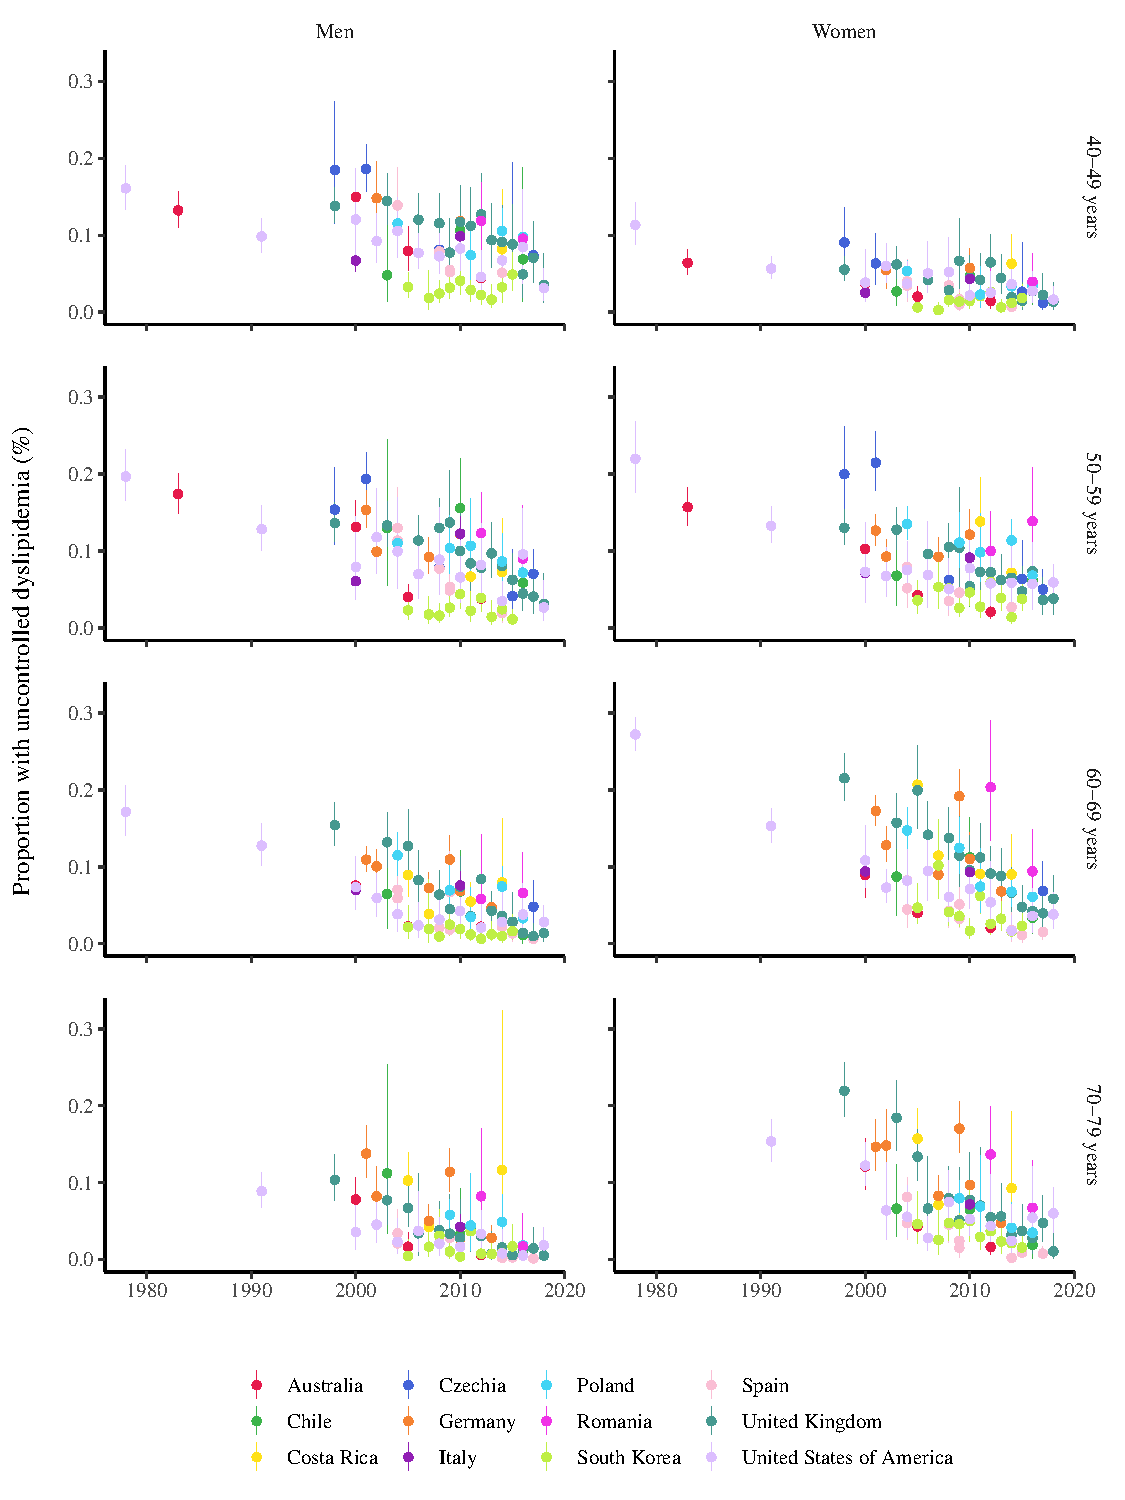
\includegraphics[width=\textwidth]{../3_figures/fig4_severe.pdf}
    \caption{Trends in uncontrolled dyslipidemia by country, sex, and age group.}
    \label{fig:severe}
\end{figure}

\begin{figure}[hp]
    \centering
    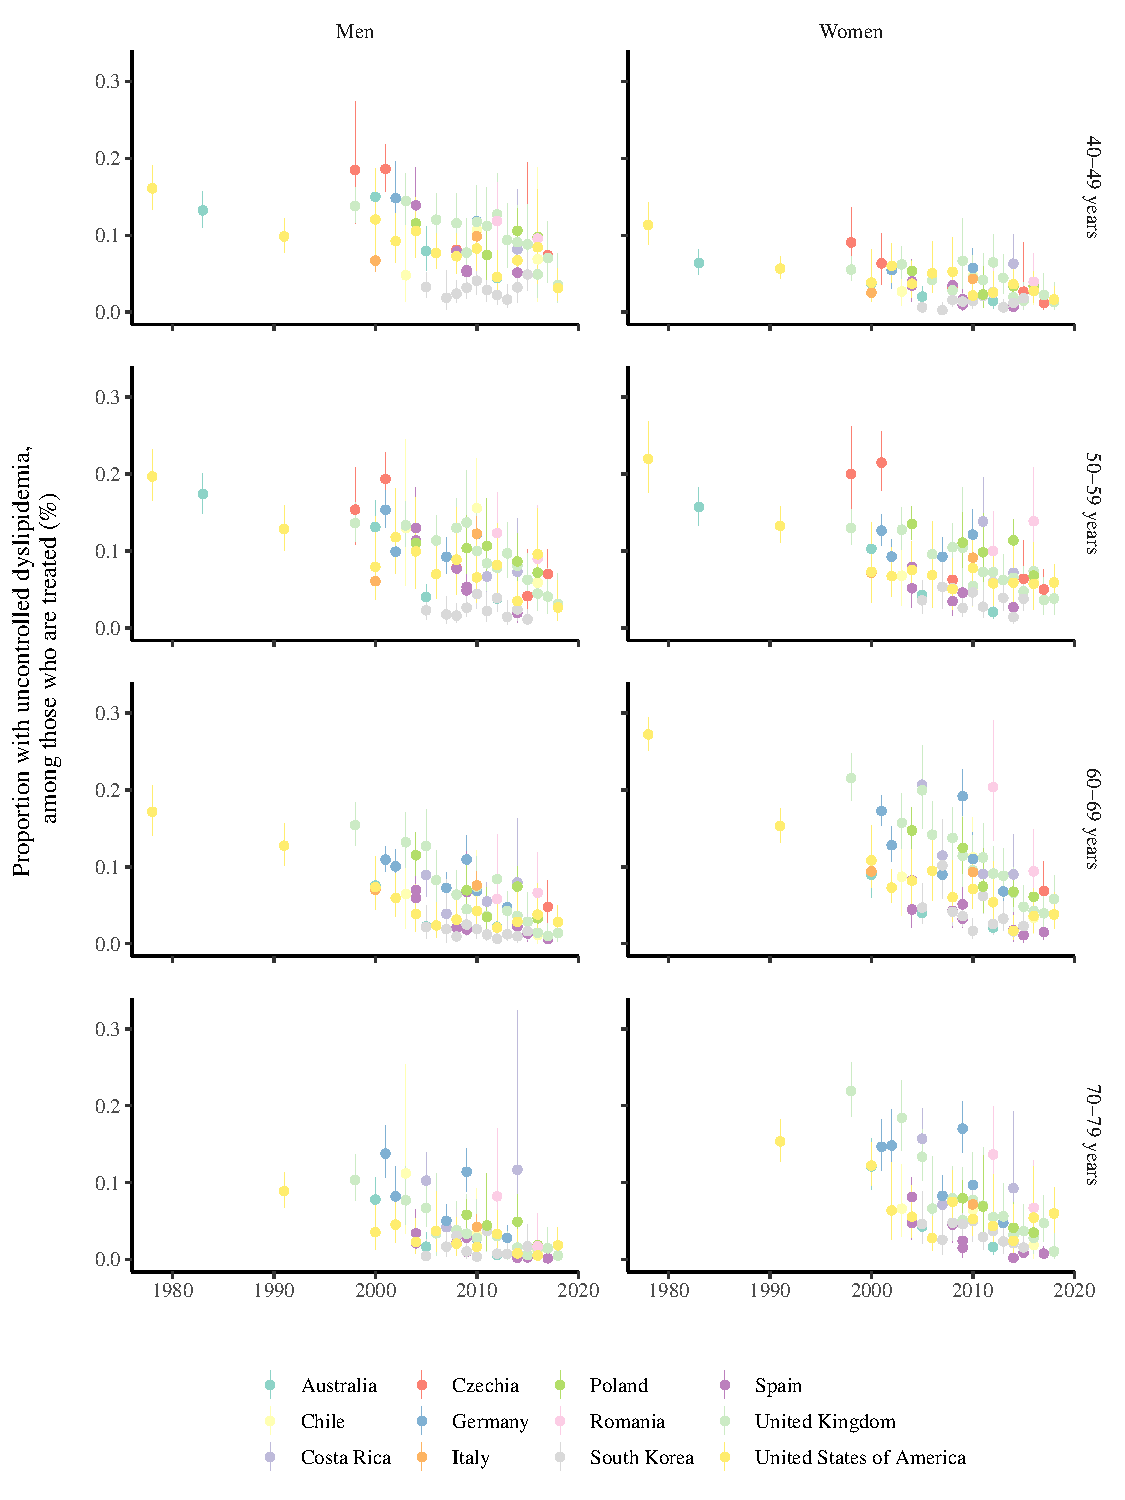
\includegraphics[width=\textwidth]{../3_figures/fig5_uncontrolled.pdf}
    \caption{Trends in uncontrolled dyslipidemia among those on treatment, by country, sex, and age group.}
    \label{fig:uncontrolled}
\end{figure}

% \begin{figure}[hp]
%     \centering
%     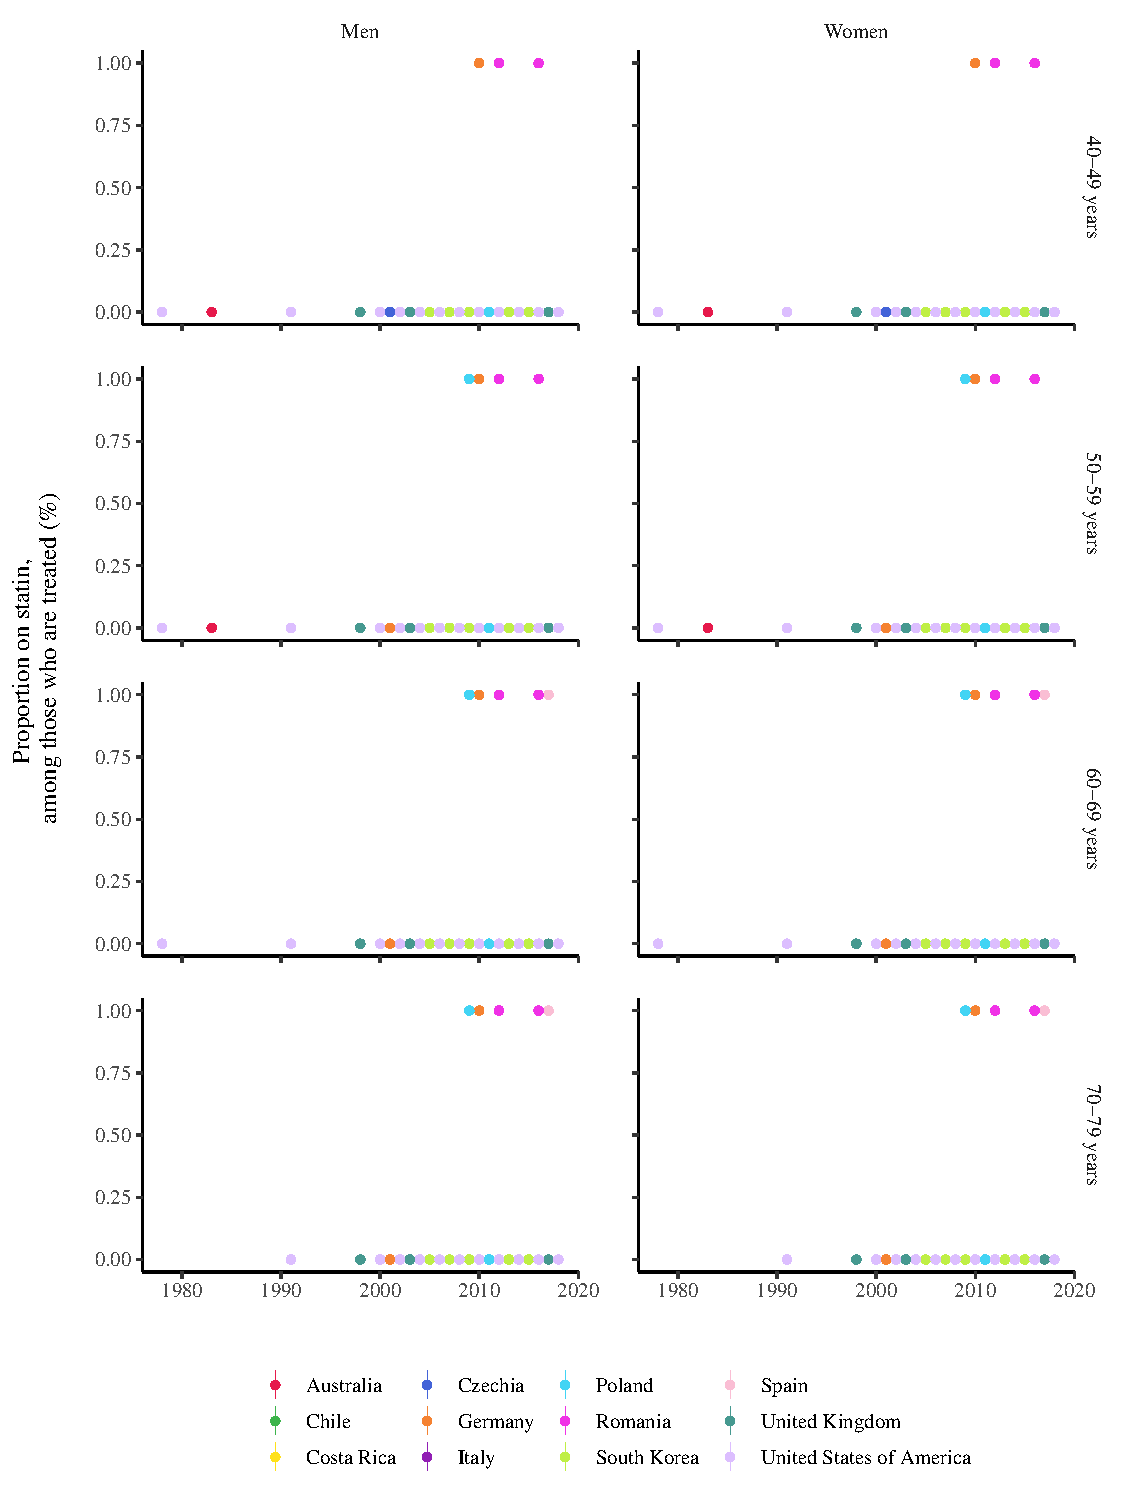
\includegraphics[width=\textwidth]{../3_figures/fig6_statin.pdf}
%     \caption{Trends in statin use among those on treatment, by country, sex, and age group.}
%     \label{fig:statin}
% \end{figure}

\clearpage
\printbibliography


\begin{appendix}
    \renewcommand{\thefigure}{A\arabic{figure}}
    \setcounter{figure}{0}
    
    \renewcommand{\thetable}{A\arabic{table}}
    \setcounter{table}{0}
    
%    \appendixwithtoc
    \newpage
    
    \section{Appendix} \label{sec:appendixa}
    \renewcommand{\thesection}{\Alph{section}}

    \subsection{Data sources}
    Using the NCDRisC database, we assembled data from 90 national health examination surveys completed between 1978 and 2018 in 12 high and middle-income countries: Australia, Chile, Costa Rica, Czech Republic, Germany, Italy, Poland, Romania, South Korea, Spain, United Kingdom, United States of America. These surveys included a lipid panel for a random sample of the general population. A list of surveys used and information about their design, including the age range and number of participants, whether LDL-C was calculated, and the devices used, is included in Table \ref{tab:data_sources}.
    
    \begin{landscape}
    \begin{singlespace}
        \begingroup\fontsize{7}{9}\selectfont

\begin{longtable}[t]{rlrrlllrr}
\caption{\label{tab:}Data sources from 12 high-income countries with laboratory lipid values}\\
\toprule
\multicolumn{5}{c}{ } & \multicolumn{2}{c}{Age range} & \multicolumn{2}{c}{Sample size} \\
\cmidrule(l{3pt}r{3pt}){6-7} \cmidrule(l{3pt}r{3pt}){8-9}
  & Country & Start & End & Survey name & Women & Men & Women & Men\\
\midrule
\endfirsthead
\caption[]{Data sources from 12 high-income countries with laboratory lipid values \textit{(continued)}}\\
\toprule
  & Country & Start & End & Survey name & Women & Men & Women & Men\\
\midrule
\endhead

\endfoot
\bottomrule
\endlastfoot
1 & Australia & 1980 & 1980 & Risk Factor Prevalence Study (RFPS) & 25-64 & 25-64 & 2756 & 2739\\
2 & Australia & 1983 & 1983 & Risk Factor Prevalence Study (RFPS) & 25-64 & 25-64 & 3732 & 3655\\
3 & Australia & 1989 & 1989 & Risk Factor Prevalence Study (RFPS) & 20-69 & 20-69 & 4611 & 4501\\
4 & Australia & 1999 & 2000 & The Australian Diabetes, Obesity and Lifestyle Study 1999-2000 (AusDiab) & 25+ & 25+ & 6138 & 5047\\
5 & Australia & 2004 & 2005 & The Australian Diabetes, Obesity and Lifestyle Study 2004-2005 (AusDiab) & 30+ & 30+ & 3444 & 2852\\
6 & Australia & 2012 & 2012 & The Australian Diabetes, Obesity and Lifestyle Study 2012 (AusDiab) & 37+ & 37+ & 2535 & 2046\\
\addlinespace
7 & Chile & 2003 & 2003 & Encuesta Nacional de Salud (ENS) & 17+ & 17+ & 1067 & 909\\
8 & Chile & 2009 & 2010 & Encuesta Nacional de Salud (ENS) & 15+ & 15+ & 1600 & 1122\\
9 & Chile & 2016 & 2017 & Encuesta Nacional de Salud (ENS) & 15+ & 15+ & 2349 & 1366\\
\addlinespace
10 & Costa Rica & 2004 & 2006 & Costa Rican Longevity and Healthy Aging Study Pre-1945 Cohort Wave 1 (CRELES) & 60+ & 60+ & 1448 & 1208\\
11 & Costa Rica & 2006 & 2008 & Costa Rican Longevity and Healthy Aging Study Pre-1945 Cohort Wave 2 (CRELES) & 62+ & 62+ & 1215 & 1018\\
12 & Costa Rica & 2010 & 2011 & Costa Rican Longevity and Healthy Aging Study 1945-1955 Cohort Wave 1 (CRELES) & 54-66 & 54-66 & 1590 & 1029\\
13 & Costa Rica & 2010 & 2010 & Costa Rican National Cardiovascular Risk Factors Survey, 2010 (CRFS) & 20+ & 20+ & 1937 & 725\\
14 & Costa Rica & 2014 & 2014 & Costa Rican National Cardiovascular Risk Factors Survey, 2014 (CRFS) & 20+ & 20+ & 1671 & 706\\
\addlinespace
15 & Czech Republic & 1992 & 1992 & MONICA, Czech Republic & 25-64 & 25-64 & 1189 & 1127\\
16 & Czech Republic & 1997 & 1998 & Czech post-MONICA (postMONICA) & 25-64 & 25-64 & 1664 & 1527\\
17 & Czech Republic & 2000 & 2001 & Czech post-MONICA (postMONICA) & 25-64 & 25-64 & 1661 & 1612\\
18 & Czech Republic & 2006 & 2009 & Czech post-MONICA (postMONICA) & 25-64 & 25-64 & 1860 & 1718\\
19 & Czech Republic & 2014 & 2015 & European Heath Examination Survey (EHES) & 25-64 & 25-64 & 681 & 472\\
20 & Czech Republic & 2015 & 2018 & MONICA & 25-65 & 25-65 & 1361 & 1239\\
\addlinespace
21 & Germany & 2000 & 2002 & ESTHER & 50-75 & 50-75 & 5270 & 4340\\
22 & Germany & 2000 & 2003 & Heinz Nixdorf Recall Study (HNRS) & 45-75 & 45-75 & 2402 & 2381\\
23 & Germany & 2005 & 2008 & Heinz Nixdorf Recall Study (HNRS) & 50-80 & 50-80 & 2082 & 2045\\
24 & Germany & 2008 & 2011 & ESTHER & 58-84 & 58-84 & 2488 & 2082\\
25 & Germany & 2008 & 2012 & Study of Health in Pomerania, second cohort (SHIP-TREND) & 20-79 & 20-79 & 2233 & 2098\\
26 & Germany & 2011 & 2014 & Heinz Nixdorf Recall Study (HNRS) & 56-85 & 56-85 & 1557 & 1492\\
\addlinespace
27 & Italy & 1998 & 2002 & Osservatorio Epidemiologico Cardiovascolare (OEC) & 35-74 & 35-74 & 4705 & 4831\\
28 & Italy & 2008 & 2012 & Osservatorio Epidemiologico Cardiovascolare/Health Examination Survey (OEC) & 35-80 & 35-80 & 4302 & 4331\\
\addlinespace
29 & Poland & 2003 & 2005 & National Multicenter Health Survey in Poland. Project WOBASZ & 20-74 & 20-74 & 6809 & 6119\\
30 & Poland & 2004 & 2004 & LIPIDOGRAM2004 Study & 30+ & 30+ & 9920 & 6672\\
31 & Poland & 2006 & 2006 & LIPIDOGRAM2006 Study & 32+ & 32+ & 10640 & 6440\\
32 & Poland & 2007 & 2011 & Medical, psychological and socioeconomic aspects of aging in Poland (PolSenior) & 55+ & 55+ & 2306 & 2427\\
33 & Poland & 2011 & 2011 & NATPOL & 18-79 & 18-79 & 1213 & 1147\\
34 & Poland & 2013 & 2014 & National Multicenter Health Survey in Poland. Project WOBASZ II & 20+ & 20+ & 3233 & 2633\\
35 & Poland & 2015 & 2016 & LIPIDOGRAM2015 \& LIPIDOGEN2015 Study & 18+ & 18+ & 8688 & 5032\\
\addlinespace
36 & Romania & 2011 & 2012 & SEPHAR II & 18-80 & 18-80 & 1037 & 931\\
37 & Romania & 2015 & 2016 & SEPHAR III & 18-80 & 18-80 & 1033 & 935\\
\addlinespace
38 & South Korea & 2005 & 2005 & Korea National Health and Nutrition Examination Survey (KNHANES) & 10+ & 10+ & 3475 & 2755\\
39 & South Korea & 2007 & 2007 & Korea National Health and Nutrition Examination Survey (KNHANES) & 10+ & 10+ & 1813 & 1388\\
40 & South Korea & 2008 & 2008 & Korea National Health and Nutrition Examination Survey (KNHANES) & 10+ & 10+ & 4142 & 3203\\
41 & South Korea & 2009 & 2009 & Korea National Health and Nutrition Examination Survey (KNHANES) & 10+ & 10+ & 4438 & 3606\\
42 & South Korea & 2010 & 2010 & Korea National Health and Nutrition Examination Survey (KNHANES) & 10+ & 10+ & 3661 & 2976\\
43 & South Korea & 2011 & 2011 & Korea National Health and Nutrition Examination Survey (KNHANES) & 10+ & 10+ & 3670 & 2888\\
44 & South Korea & 2012 & 2012 & Korea National Health and Nutrition Examination Survey (KNHANES) & 10+ & 10+ & 3461 & 2691\\
45 & South Korea & 2013 & 2013 & Korea National Health and Nutrition Examination Survey (KNHANES) & 10+ & 10+ & 3219 & 2635\\
46 & South Korea & 2014 & 2014 & Korea National Health and Nutrition Examination Survey (KNHANES) & 10+ & 10+ & 3025 & 2365\\
47 & South Korea & 2015 & 2015 & Korea National Health and Nutrition Examination Survey (KNHANES) & 10+ & 10+ & 3080 & 2568\\
\addlinespace
48 & Spain & 1991 & 1993 & Cardiovascular Risk Factors Survey in Murcia (CVDRF) & 18-69 & 18-69 & 1268 & 1151\\
49 & Spain & 2003 & 2005 & Registre Gironi del Cor (REGICOR) & 35-79 & 35-79 & 3280 & 2951\\
50 & Spain & 2004 & 2006 & PREVICTUS & 60+ & 60+ & 3834 & 3350\\
51 & Spain & 2004 & 2004 & Cardiovascular Risk Study in Castilla y León (RECCyL) & 15+ & 15+ & 2069 & 1897\\
52 & Spain & 2007 & 2009 & Harmonizing Equation of Risk in Mediterraneon countries EXtremadura (HERMEX) & 25-79 & 25-79 & 1498 & 1297\\
53 & Spain & 2008 & 2010 & Study on Nutrition and Cardiovascular Risk in Spain (ENRICA) & 18+ & 18+ & 6858 & 6193\\
54 & Spain & 2009 & 2009 & Cardiovascular Risk Study in Castilla y León (RECCyL) & 20+ & 20+ & 1572 & 1291\\
55 & Spain & 2014 & 2014 & Cardiovascular Risk Study in Castilla y León (RECCyL) & 20+ & 20+ & 1509 & 1220\\
56 & Spain & 2015 & 2015 & Study on Nutrition and Cardiovascular Risk in Spain (ENRICA) & 65+ & 65+ & 770 & 704\\
\addlinespace
57 & United Kingdom & 1986 & 1987 & Dietary and Nutritional Survey of British Adults 1986-1987 (DNS) & 16-64 & 16-64 & 937 & 936\\
58 & United Kingdom & 1998 & 1998 & Health Survey for England (HSE) & 16+ & 16+ & 5565 & 5000\\
59 & United Kingdom & 2003 & 2003 & Health Survey for England (HSE) & 16+ & 16+ & 4460 & 3814\\
60 & United Kingdom & 2005 & 2005 & Health Survey for England (HSE) & 65+ & 65+ & 1190 & 1008\\
61 & United Kingdom & 2006 & 2006 & Health Survey for England (HSE) & 16+ & 16+ & 4061 & 3409\\
62 & United Kingdom & 2008 & 2008 & Health Survey for England (HSE) & 16+ & 16+ & 3922 & 3348\\
63 & United Kingdom & 2008 & 2012 & National Diet and Nutrition Survey (NDNS) & 10+ & 10+ & 1266 & 1008\\
64 & United Kingdom & 2009 & 2009 & Health Survey for England (HSE) & 16+ & 16+ & 1227 & 1075\\
65 & United Kingdom & 2010 & 2010 & Health Survey for England (HSE) & 16+ & 16+ & 2158 & 1720\\
66 & United Kingdom & 2011 & 2011 & Health Survey for England (HSE) & 16+ & 16+ & 2201 & 1738\\
67 & United Kingdom & 2012 & 2012 & Health Survey for England (HSE) & 16+ & 16+ & 2192 & 1745\\
68 & United Kingdom & 2013 & 2013 & Health Survey for England (HSE) & 16+ & 16+ & 2438 & 2080\\
69 & United Kingdom & 2013 & 2014 & National Diet and Nutrition Survey (NDNS) & 10+ & 10+ & 520 & 386\\
70 & United Kingdom & 2014 & 2014 & Health Survey for England (HSE) & 16+ & 16+ & 2085 & 1816\\
71 & United Kingdom & 2015 & 2015 & Health Survey for England (HSE) & 16+ & 16+ & 2130 & 1777\\
72 & United Kingdom & 2015 & 2016 & National Diet and Nutrition Survey (NDNS) & 10+ & 10+ & 485 & 391\\
73 & United Kingdom & 2016 & 2016 & Health Survey for England (HSE) & 16+ & 16+ & 2083 & 1682\\
74 & United Kingdom & 2016 & 2017 & National Diet and Nutrition Survey (NDNS) & 10+ & 10+ & 204 & 174\\
75 & United Kingdom & 2017 & 2017 & Health Survey for England (HSE) & 16+ & 16+ & 2160 & 1711\\
76 & United Kingdom & 2018 & 2018 & Health Survey for England (HSE) & 16+ & 16+ & 1947 & 1600\\
\addlinespace
77 & United States of America & 1976 & 1980 & US NHANES II & 20-74 & 20-74 & 6245 & 5601\\
78 & United States of America & 1988 & 1994 & US NHANES III & 10+ & 10+ & 10275 & 9408\\
79 & United States of America & 1999 & 2000 & US NHANES 1999-2000 & 10+ & 10+ & 3123 & 3150\\
80 & United States of America & 2001 & 2002 & US NHANES 2001-2002 & 10+ & 10+ & 3402 & 3496\\
81 & United States of America & 2003 & 2004 & US NHANES 2003-2004 & 10+ & 10+ & 3202 & 3361\\
82 & United States of America & 2005 & 2006 & US NHANES 2005-2006 & 10+ & 10+ & 3128 & 3302\\
83 & United States of America & 2007 & 2008 & US NHANES 2007-2008 & 10+ & 10+ & 3333 & 3367\\
84 & United States of America & 2009 & 2010 & US NHANES 2009-2010 & 10+ & 10+ & 3599 & 3558\\
85 & United States of America & 2011 & 2012 & US NHANES 2011-2012 & 10+ & 10+ & 3131 & 3155\\
86 & United States of America & 2013 & 2014 & US NHANES 2013-2014 & 10+ & 10+ & 3535 & 3350\\
87 & United States of America & 2015 & 2016 & US NHANES 2015-2016 & 10+ & 10+ & 3320 & 3218\\
88 & United States of America & 2017 & 2018 & US NHANES 2017-2018 & 10+ & 10+ & 3153 & 3011\\*
\end{longtable}
\endgroup{}

        \label{tab:data_sources}
    \end{singlespace}
    \end{landscape}


    \subsection{Data cleaning}
    Given the heterogeneity in the data collection procedures and cleaning across surveys, we implemented a secondary data cleaning protocol, developed for NCD-RisC, and applied it to the pooled data from all 90 surveys. The basic steps were as follows, we evaluated:
    \begin{enumerate}
        \item univariate plausibility ranges
        \item multivariate plausibility constraints
        \item multivariate outlier detection
    \end{enumerate}

    \subsubsection{Univariate plausibility ranges}
    We removed values of certain laboratory and examination measurements that were outside the range of biological plausibility, as determined by expert consensus. Table \ref{tab:plausibility} below shows the plausiblity ranges used for each variable.

    \begin{table}[H]
        \centering
        \caption{Univariate plausibility ranges for select variables from national surveys.}
        \begin{tabular}{lcc}
            \hline
            Variable & Ages & Plausibility range \\
            \hline
            height (cm) & 5 to 9 years & 60 - 180 \\
            height (cm) & 10 to 14 years & 80 - 200 \\
            height (cm) & $\geq$15 years & 100 - 250 \\
            weight (kg) & 5 to 9 years & 5 - 90 \\
            weight (kg) & 10 to 14 years & 8 - 150 \\
            weight (kg) & $\geq$15 years & 12 - 300 \\
            BMI (kg/m$^2$) & 5 to 9 years & 6 - 40 \\
            BMI (kg/m$^2$) & 10 to 14 years & 8 - 60 \\
            BMI (kg/m$^2$) & $\geq$15 years & 10 - 80 \\
            SBP (mmHg) & all & 70 - 270 \\
            DBP (mmHg) & all & 30 - 150 \\
            TC (mmol/L) & all & 1.75 - 20 \\
            LDL (mmol/L) & all & 0.5 - 10 \\
            HDL (mmol/L) & all & 0.4 - 5 \\
            Triglycerides (mmol/L) & all & 0.2 - 20 \\
            \hline
        \end{tabular}
        \label{tab:plausibility}
    \end{table}

    \subsubsection{Multivariate plausibility constraints}
    After removing data outside the univariate plausibilty ranges, we also apply logical multivariate biological plausibility constraints such as checking that the reported systolic blood pressure measurement is greater than the diastolic measurement. We evaluated the following constraints:
    \begin{itemize}
        \item SBP $>$ DBP (before calculating average BP) 
        \item TC $>$ LDL 
        \item TC $>$ HDL
        \item TC – (LDL + HDL) $\geq$ margin of error\footnote{“margin of error” is determined by using the Cholesterol Reference Method Laboratory Network permitted measurement error limits for TC (8.9\%), HDL (13\%) and LDL (12\%) as follows: Calculate errors in worst case scenario, i.e., TC underestimated, and HDL/LDL overestimated, each by the largest error permitted.}
    \end{itemize}
    Table \ref{tab:mv_constraints} below shows the number of implausible observations identified and set to missing.
    \begin{table}[H]
        \centering
        \caption{Implausible values detected using mulitvariate biological plausibility constraints.}
        \label{tab:mv_constraints}
        \begin{tabular}{lccc}
            \toprule
            Constraint & Evaluated (N) & Implausible (N) & \% \\
            \midrule
            DBP $>$ SPB & 478,407 & 8 & 0.002\\
            LDL $>$ TC & 274,214 & 36 & 0.013\\
            HDL $>$ TC & 459,919 & 4 & 0.001\\
            TC – (LDL + HDL) $\geq$ margin of error & 273,547 & 209 & 0.076\\
            \bottomrule
            \end{tabular}
    \end{table}

    \subsubsection{Multivariate outlier detection}
    Finally, we identify multivariate outliers across pairwise combinations of risk factors based on the Mahalanobis distance. That is for vectors of observations for variables $\mathbf{x}$ and $\mathbf{y}$ we calculate the distance
    $$d(\mathbf{x}, \mathbf{y}) = \sqrt{(\mathbf{x} - \mathbf{y})^t \Sigma (\mathbf{x} - \mathbf{y})}$$
    where $\Sigma$ is the covariance matrix, which gives a sense for how far a paired set of values is from the multivariate center. For skewed variables we apply a log transformation prior to the calculation of the Mahalanobis distance. To identify potentially implausible combinations of values, we use a cut-off based on quantiles of the $\chi^2$ distribution, corresponding to a combination being more the 6 standard deviations from the center. Figure \ref{fig:pairs} below plots the pairwise distributions and highlights the possible outliers identified. 

    \begin{figure}[H]
        \centering
        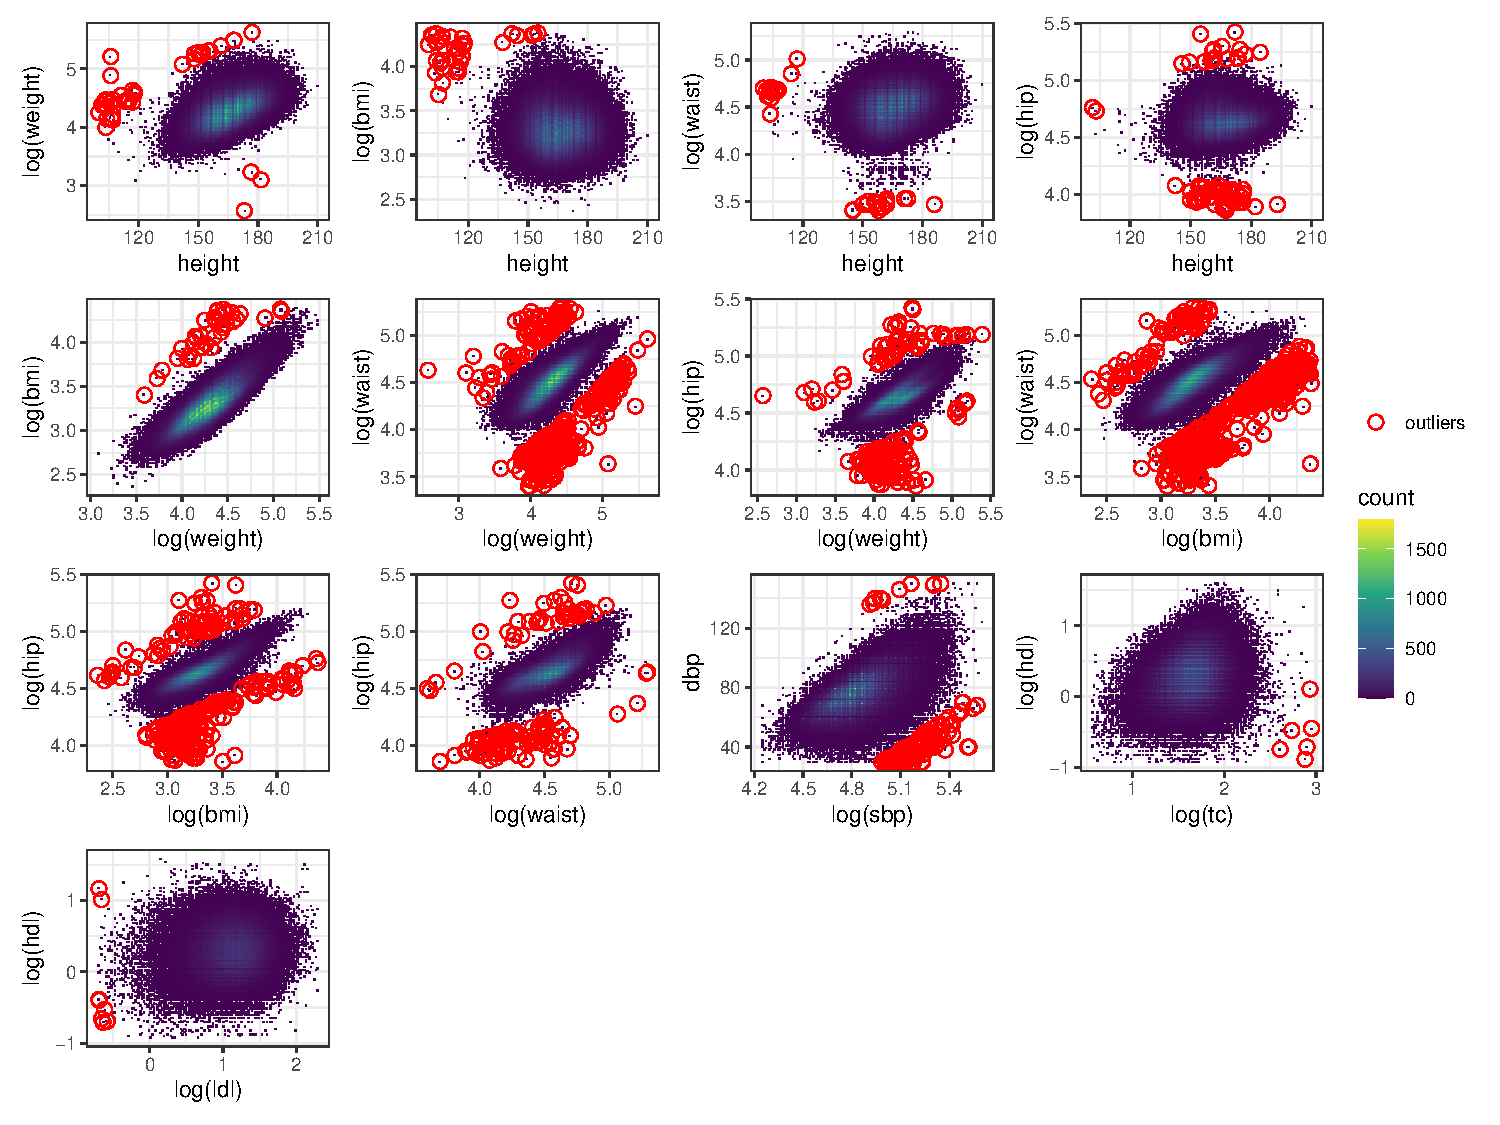
\includegraphics[width = \linewidth]{../3_figures/figS2_maha_outliers.pdf}
        \caption{Pairwise outliers based on Mahalanobis distance}
        \label{fig:pairs}
    \end{figure}

    \begin{table}[H]
        \centering
        \caption{Pairwise outliers detected using Mahalanobis distance.}
        \begin{tabular}{lccc}
            \toprule
            Variable Pair & Evaluated (N) & Outliers (N) & \% \\
            \midrule
            HEIGHT vs. WEIGHT & 530,247 & 45 & 0.0084\\
            HEIGHT vs. BMI & 530,223 & 32 & 0.0060\\
            HEIGHT vs. WAIST & 441,684 & 32 & 0.0072\\
            HEIGHT vs. HIP & 259,229 & 71 & 0.0273\\
            WEIGHT vs. BMI & 530,223 & 36 & 0.0067\\
            WEIGHT vs. WAIST & 441,837 & 410 & 0.0927\\
            WEIGHT vs. HIP & 259,232 & 179 & 0.0690\\
            BMI vs. WAIST & 439,276 & 493 & 0.1122\\
            BMI vs. HIP & 257,094 & 246 & 0.0956\\
            WAIST vs. HIP & 265,771 & 115 & 0.0432\\
            SBP vs. DBP & 476,122 & 100 & 0.0210\\
            TC vs. HDL & 459,027 & 6 & 0.0013\\
            LDL vs. HDL & 273,370 & 13 & 0.0047\\
            \bottomrule
            \end{tabular}
    \end{table}

    \subsection{Exclusion criteria}
    The flow diagram below shows how we arrived at our final analytic sample. First, we excluded 191,912 subjects outside our target age range of 40-79 years of age, as this population is generally the focus of cholesterol treatment guidelines for primary and secondary prevention. Next, we excluded 9,120 subjects in 10-year age groups from surveys in which we had less than 5 of the 10 ages observed. Finally, we excluded 77,165 subjects with missing data on cholesterol levels and 58,999 subjects with missing data on key risk factors for calculating risk thresholds, leaving a final sample of 255,369.
    \begin{figure}[H]
        \centering
        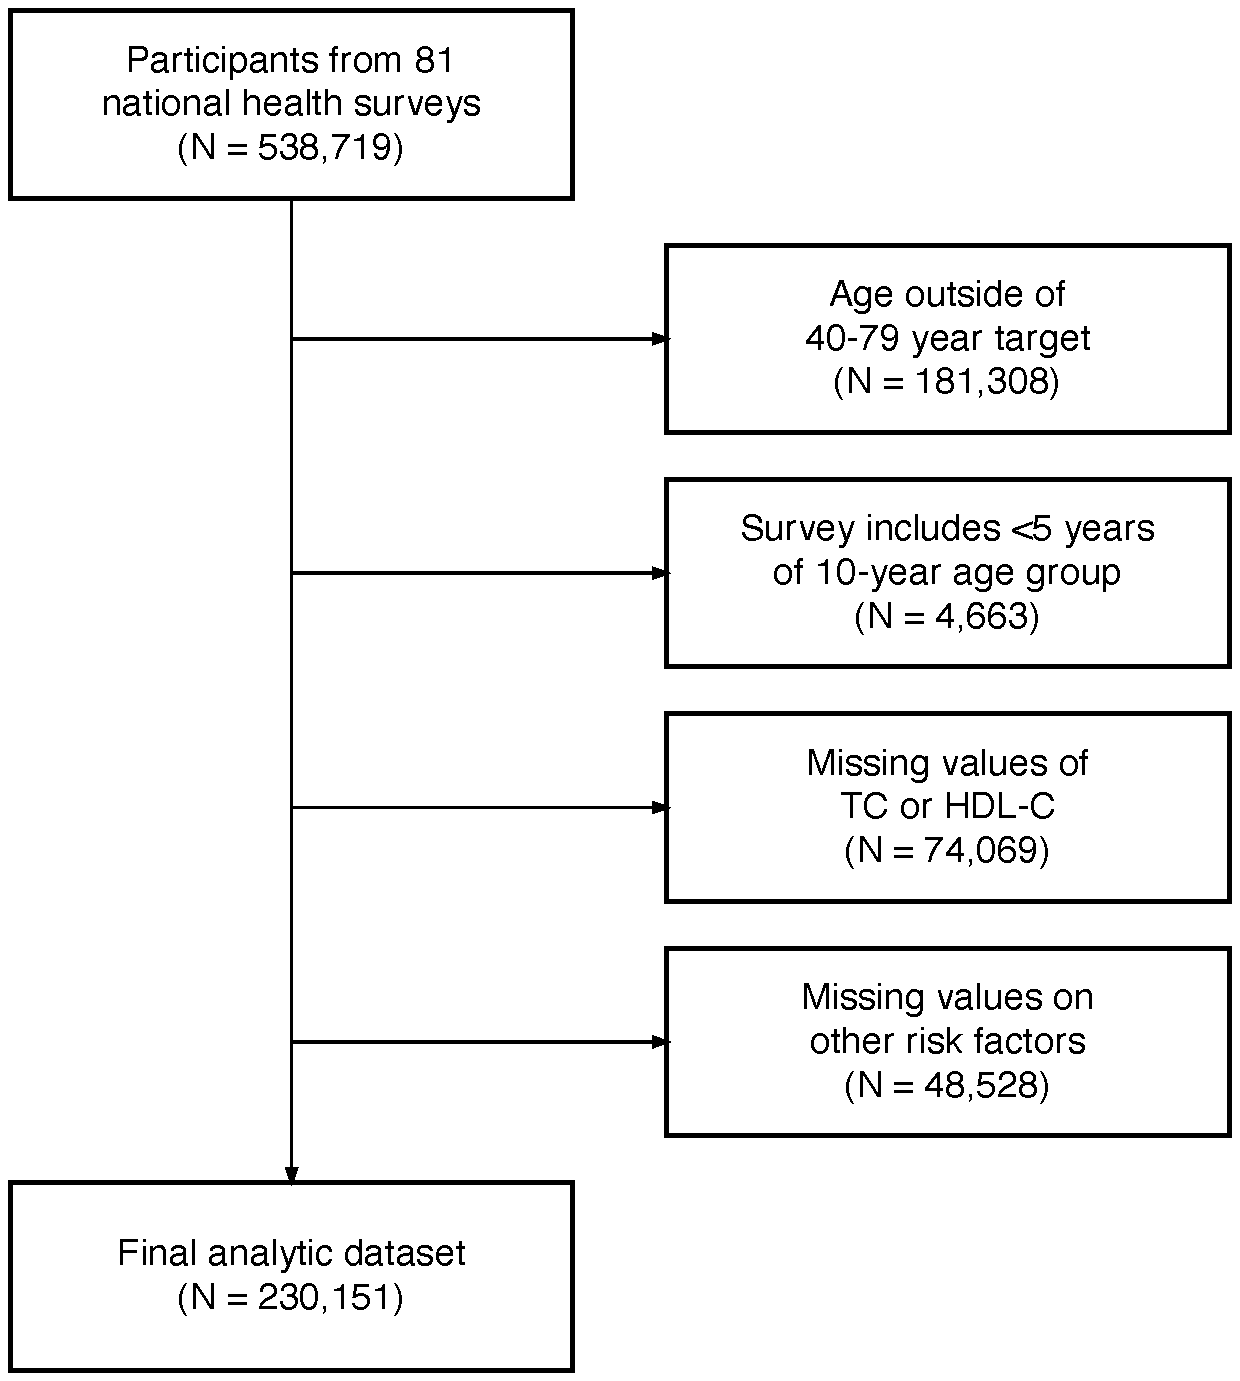
\includegraphics[width=0.5\linewidth]{../3_figures/figS_STROBE.pdf}
        \caption{Exclusion criteria.}
        \label{fig:exclusion}
    \end{figure}

    \subsection{Cholesterol Treatment Guidelines}

    We compiled a list of cholesterol treatment guidelines from official sources that have been published and discussed in the academic literature. Most of these come from a review conducted by the World Heart Foundation in 2019. They were used as criteria for determining who should be on treatment in assembled surveys. Note that many of these same sources have guidance about control as well (i.e. ideal reductions in LDL or absolute level attained while on treatment). Table \ref{tab:guidelines} below summarizes the specific treatment guidance from the US, Europe, the UK, Canada, China, Brazil, South Africa, and the WHO. 

    For this study, we based our definition of treatment eligibility on the NHLBI NCEP ATP III guidelines to define the eligible population as those meeting:
    \begin{itemize}
        \item Non-HDL-C $>$ 220 mg/dL (LDL-C $>$ 190 mg/dL) or
        \item Non-HDL-C $>$ 190 mg/dL (LDL-C $>$ 160 mg/dL) and 10-year risk $>$ 5\% or
        \item Non-HDL-C $>$ 145 mg/dL (LDL-C $>$ 130 mg/dL) and 10-year risk $>$ 10\% or
        \item Non-HDL-C $>$ 115 mg/dL (LDL-C $>$ 100 mg/dL) and 10-year risk $>$ 20\% or
        \item Already on cholesterol lowering medication
    \end{itemize}
    where the last criteria assumes that those already on lipid-lowering medication were eligible at the time the meds were perscribed. As described below we used Globorisk risk equations to calculate CVD risk to inform eligibility.

\begin{landscape}
    \begin{table}[H]
        \centering
        \caption{Cholesterol treatment guidelines and recommendations for primary prevention.}
        \tiny{
        \begin{threeparttable}
        \begin{tabular}{llll}
            \toprule
            Source & Year & Treatment recommendation & Goal of therapy\\
            \midrule  
            %  \hline
            NHLBI NCEP ATP III \cite{noauthor_third_2002} & 2013 & LDL $\geq 100$ mg/dL and 10-year risk\tnote{*} \hspace{1pt}  $\geq$ 20\%  & LDL $<$ 100 mg/dL \\
            & & LDL $\geq 130$ mg/dL and 10-year risk\tnote{*} \hspace{1pt}  $\geq$ 10\% (2+ risk factors) & LDL $<$ 130 mg/dL  \\
            & & LDL $\geq 160$ mg/dL and 10-year risk\tnote{*} \hspace{1pt}  $<$ 10\% (2+ risk factors) & LDL $<$ 130 mg/dL  \\
            & & LDL $\geq 190$ mg/dL (0-1 risk factors) & LDL $<$ 160 mg/dL \\
            & & & \\
            %  \hline
            AHA/ACC Statement \cite{grundy_scott_m_2018_2019} & 2018 & LDL $\geq 190$ mg/dL (severe hypercholesterolemia) & LDL $<$ 100 mg/dL \\
            & & LDL $\geq 70$ mg/dL and 10-year risk\tnote{*} \hspace{1pt}  $\geq$ 7.5\%  & LDL reduced 30\% to 49\%\\
            & & LDL $\geq 70$ mg/dL and 10-year risk\tnote{*} \hspace{1pt}  $\geq$ 20\% & LDL reduced $\geq$ 50\%\\
            & & LDL $\geq 70$ mg/dL and diabetes mellitus & LDL reduced $\geq$ 50\% \\
            & & & \\
            ESC/EAS Guidelines \cite{mach_2019_2020} & 2019 & LDL $\geq 70$ mg/dL and 10-year risk\tnote{\textdagger} \hspace{1pt} $\geq$ 10\% (very-high) & LDL reduced $\geq$ 50\% or $<$ 55 mg/dL \\
            & & LDL $\geq 100$ mg/dL and 10-year risk\tnote{\textdagger} \hspace{1pt}  $\geq$ 5\% (high) & LDL reduced $\geq$ 50\% or $<$ 70 mg/dL \\
            & & LDL $\geq 190$ mg/dL and 10-year risk\tnote{\textdagger} \hspace{1pt}  $\geq$ 1\% (moderate) & LDL $<$ 100 mg/dL \\
            & & LDL $\geq 190$ mg/dL and 10-year risk\tnote{\textdagger} \hspace{1pt} $<$ 1\% (low) & LDL $<$ 116 mg/dL \\
            & & & \\
            NICE Guidelines \cite{rabar_lipid_2014} & 2014 & 10-year risk\tnote{\ddag} \hspace{1pt} $\geq$ 10\% or CKD &  \\
            & & diabetes mellitus (type-2) and 10-year risk\tnote{\ddag} \hspace{1pt} $\geq$ 10\% &  \\
            & & diabetes mellitus (type-1), $>$40 years-old, duration $>$10 years &  \\
            & & & \\
            CCS Guidelines \cite{anderson_2012_2013} & 2012 & LDL $\geq 75$ mg/dL and 10-year risk\tnote{\S} \hspace{1pt} $\geq$ 20\% & LDL $<$ 75 mg/dL \\
            & & LDL $\geq 130$ mg/dL and 10-year risk\tnote{\S} \hspace{1pt}  $\geq$ 10\% & LDL $<$ 130 mg/dL \\
            & & LDL $\geq 130$ mg/dL and 10-year risk\tnote{\S} \hspace{1pt}  $\geq$ 5\% (optional) & LDL $<$ 190 mg/dL \\
            & & LDL $\geq 190$ mg/dL and 10-year risk\tnote{\S} \hspace{1pt} $<$ 1\% & LDL $<$ 190 mg/dL \\
            & & & \\
            China Guidelines \cite{anderson_2012_2013} & 2016 & 10-year risk\tnote{$||$} \hspace{1pt} $\geq$ 10\% & LDL $<$ 130 mg/dL \\
            & & 10-year risk\tnote{$||$} \hspace{1pt} $\geq$ 5\% & LDL $<$ 130 mg/dL \\
            & & diabetes mellitus and LDL $\geq 70$ mg/dL or TC $\geq 120$ & LDL $<$ 100 mg/dL \\
            & & LDL $\geq 190$ mg/dL or TC $\geq 280$ & LDL $<$ 100 mg/dL \\
            & & & \\
            Brazil Guidelines \cite{anderson_2012_2013} & 2013 & 10-year risk\tnote{\S} \hspace{1pt} $\geq$ 10\% (women) $\geq$ 20\% (men) & LDL $<$ 100 mg/dL \\
            & & diabetes mellitus or CKD or FH & LDL $<$ 70 mg/dL \\
            & & & \\
            South Africa Guidelines \cite{anderson_2012_2013} & 2012 & 10-year risk\tnote{\S} \hspace{1pt} $\geq$ 30\% (very high) & LDL $<$ 70 mg/dL \\
            & & LDL $\geq 100$ mg/dL and 10-year risk\tnote{\S} \hspace{1pt}  $\geq$ 15\% (high) & LDL $<$ 100 mg/dL \\
            & & diabetes mellitus or CKD or FH & LDL $<$ 70 mg/dL \\
            & & & \\
            WHO Guidelines \cite{anderson_2012_2013} & 2007 & TC $\geq$ 320 mg/dL or LDL $\geq$ 240 mg/dL or TC/HDL ratio $>$ 8 & LDL $<$ 77 mg/dL or TC $<$ 152 mg/dL \\
            & & diabetes mellitus & LDL $<$ 77 mg/dL or TC $<$ 152 mg/d  \\
            & & 10-year risk\tnote{\P} \hspace{1pt} $\geq$ 30\% & LDL $<$ 77 mg/dL or TC $<$ 152 mg/dL \\
            & & LDL $\geq 115$ mg/dL or TC $\geq 193$ mg/dL and 10-year risk\tnote{\P} \hspace{1pt}  $\geq$ 20\% & LDL $<$ 100 mg/dL \\
            \bottomrule
        \end{tabular}
        \begin{tablenotes}
            \item[*] Based on Pooled Cohort Equations
            \item[\textdagger] Based on SCORE
            \item[\ddag] Based on QRISK2
            \item[\S] Based on Framingham Risk Score
            \item[$||$] Based on CMCS re-callibration
            \item[\P] Based on WHO/ISH risk charts
        \end{tablenotes}
        \end{threeparttable}
        }
        \label{tab:guidelines}
    \end{table}

\end{landscape}
    
    \newpage

    \subsection{Calibrating Non-HDL-C to LDL-C}
    In this study, we use non-HDL-C to define those who are elligible for treatment with lipid-lowering drugs as well as those whose serum cholesterol levels are ``controlled''. However, most national guidelines use LDL-C targets rather than non-HDL-C. We chose to use non-HDL-C because many surveys, especially those conducted several decades ago, did not measure LDL-C or did not measure the necessary components\footnote{Roughly speaking total cholesterol is composed of HDL-C, LDL-C, and Triglycerides} to calculate LDL-C. In the main text, we use a correction factor to convert LDL-C targets in guidelines to non-HDL-C derived from more recent guidelines in Europe and North America. 
    
    Here we validate this correction factor in our sample by looking at the relationship between non-HDL-C and LDL-C among studies in which both were measured (N = 198,761 observations). Figure \ref{fig:callibration} below plots non-HDL-C levels versus LDL-C levels. We fit both a linear as well as a more flexbile GAM regression model to the data and find evidence that the relationship is linear across the full range. We find a high degree of linear correlation between non-HDL-C and LDL-C ($\rho = 0.916$) with an estimated bias/correction factor of 0.65 mmol/L (25.2 mg/dL) which compares favorably with the one in the literature of 0.78 mmol/L (30 mg/dL).

    \begin{figure}[H]
    \centering
    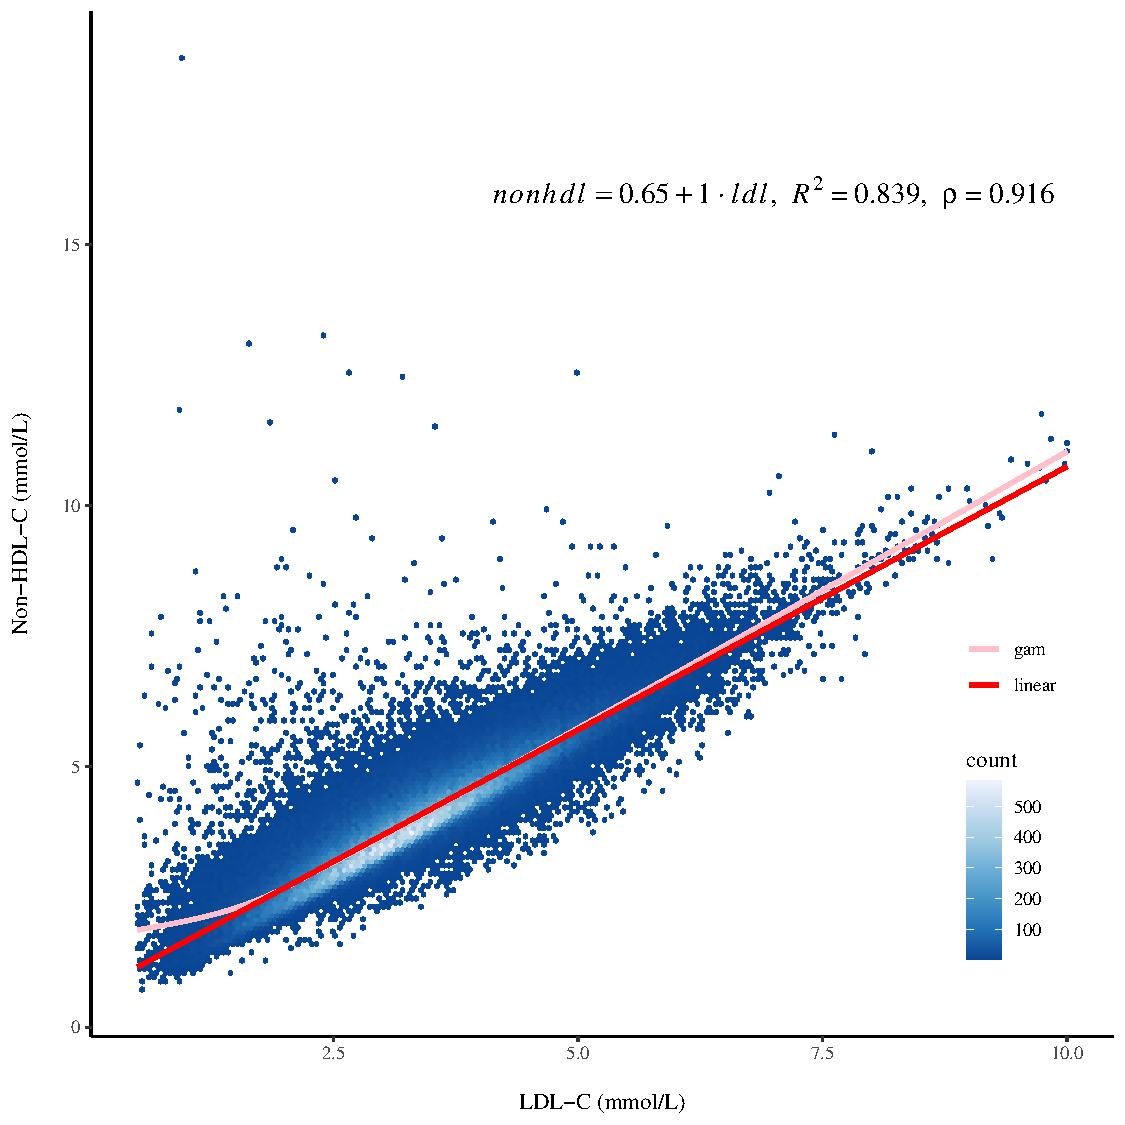
\includegraphics[width=\textwidth]{../3_figures/figS1_calibration.pdf}
    \caption{Callibrating non-HDL-C levels with LDL-C among those surveys which collected data on both.}
    \label{fig:callibration}
    \end{figure}

    \newpage 

    \subsection{Calculation of risk scores}
    For risk-based guidelines about treatment eligibility, we used Globorisk \cite{hajifathalian_novel_2015} to calculate risk scores for all individuals with complete risk factor data. Globorisk is a cardiovascual disease risk prediction equation that can be recalibrated and updated for use in different countries with routinely available information. Currently it supports risk estimates for 182 countries from 2000 to 2020 \cite{ueda_laboratory-based_2017}. Coefficients were estimated in original study using Cox propostional hazards model with age as the time scale. Thus the risk equation is of the form: 
    
    \begin{align*}
        h(t \mid& sex, sbp, tc, dm, smk) = h_0(t) \exp\big\{ \\
        &\quad \beta_1 (sbp - \overline{sbp}) + \beta_2 (tc - \overline{tc}) + \beta_3 (dm - \overline{dm}) + \beta_4 (smk - \overline{smk}) + \beta_5 (dm - \overline{dm}) \times sex
        \\ &\quad + \beta_6 (smk - \overline{smk}) \times sex + \beta_7 (sbp - \overline{sbp}) \times t + \beta_8 (tc - \overline{tc}) \times t + \beta_9 (dm - \overline{dm}) \times t
        \\ &\quad  + \beta_{10} (smk - \overline{smk}) \times t \\
        \big\}
    \end{align*}
    where $(\beta_1, \ldots, \beta_{10})$ are constant across countries but the mean risk factor levels $(\overline{sbp}, \ldots, \overline{smk}$) and baseline hazard $h_0(t)$ are country-specific and thus can be re-callibrated to local conditions. The values of $(\beta_1, \ldots, \beta_{10})$ are provided in table below.
    \begin{table}[H]
        \centering
        \caption{Coefficient values for Globorisk risk equations.}
        \label{tab:coefs}
        \begin{tabular}[t]{cc}
            \toprule
            Coefficient & Estimate  \\
            \midrule
            $\beta_1$ & 0.3070129 \\
            $\beta_2$ & 0.6149061 \\
            $\beta_3$ & 1.475305 \\
            $\beta_4$ & 1.846684 \\
            $\beta_5$ & 0.4050458 \\
            $\beta_6$ & 0.3253832 \\
            $\beta_7$ & -0.002247118 \\
            $\beta_8$ & -0.006865652 \\
            $\beta_9$ & -0.01320953 \\
            $\beta_{10}$ & -0.02205285 \\
            \bottomrule
            \end{tabular}
    \end{table}
    Country-specific risk factor values and baseline hazards were the same as those used in a prior study \cite{ueda_laboratory-based_2017}. The estimated risk for each subject is calculated as 10-year cumulative incidence based on the formula
    \begin{equation*}
        CI = 1 - \prod_{t=0}^T\exp\{h(t \mid sex, sbp, tc, dm, smk)\}.
    \end{equation*}
    All calculations were performed using the \texttt{globorisk} package \cite{boyer_globorisk_2022} in R. For reference, below are the trends in mean risk score by country, sex, and age group. 

    \begin{figure}[hp]
        \centering
        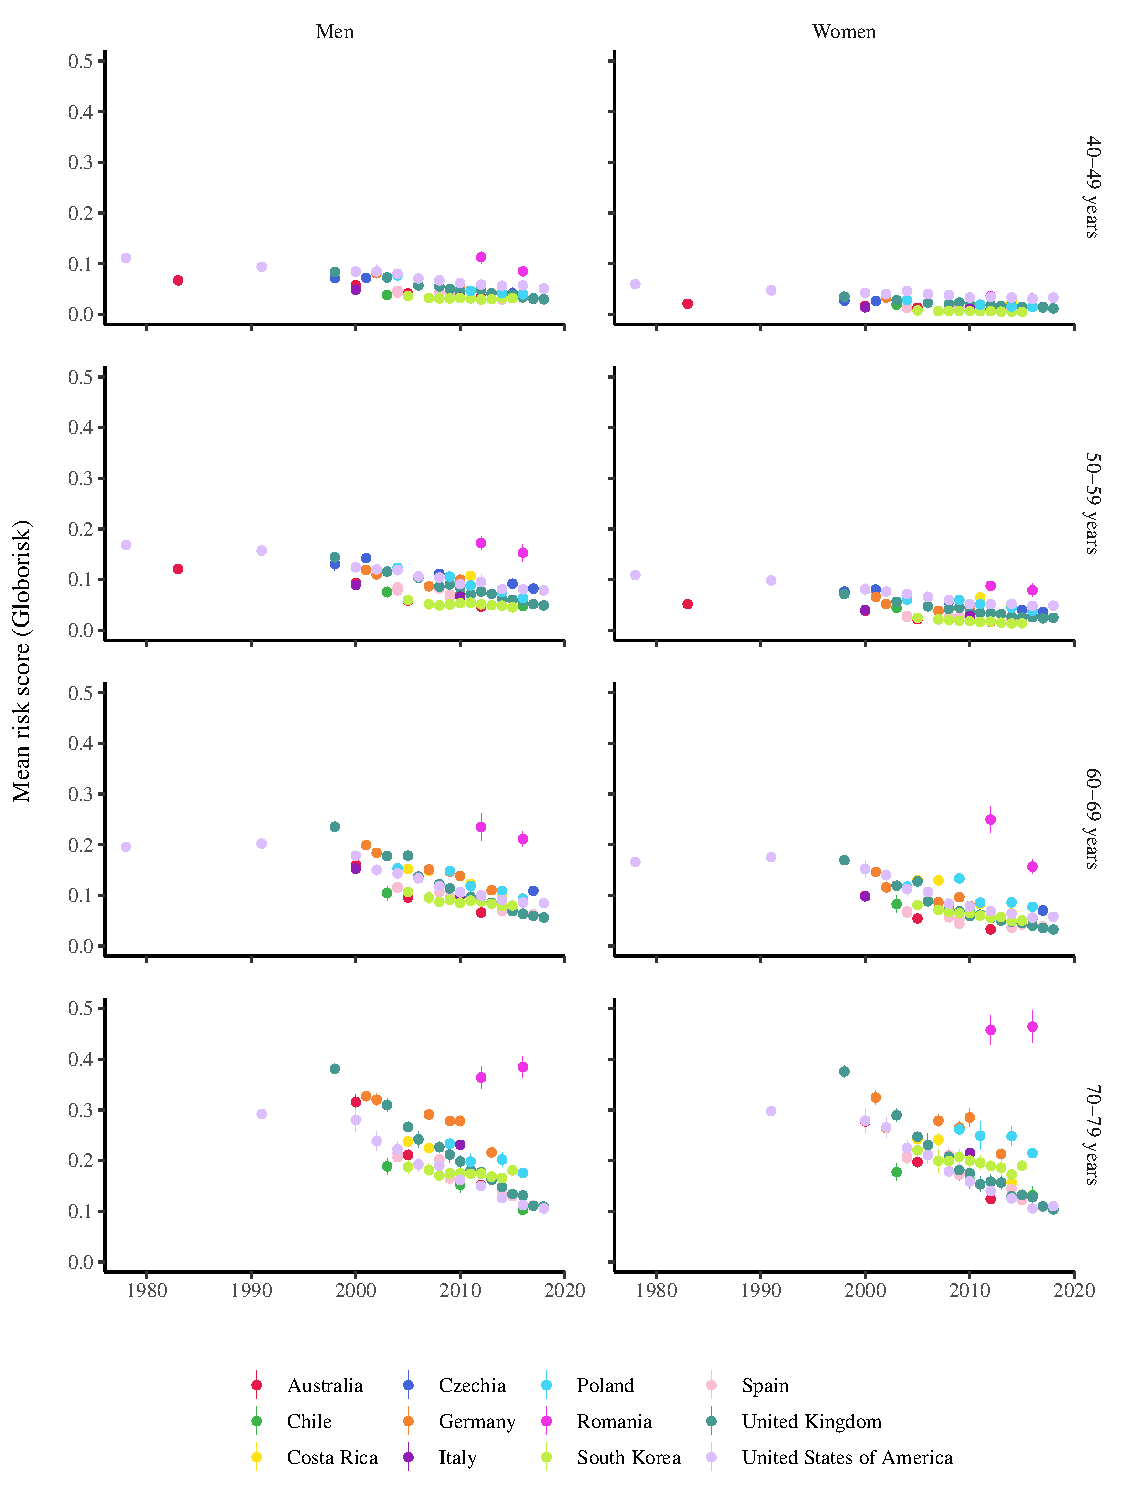
\includegraphics[width=\textwidth]{../3_figures/figS3_risk_score.pdf}
        \caption{Trends in mean risk score by country, sex, and age group.}
        \label{fig:globorisk}
    \end{figure}
    
%    \subsection{Sensitivity analyses}

    \newpage
    \subsection{Linear trends}

    \begin{figure}[H]
        \centering
        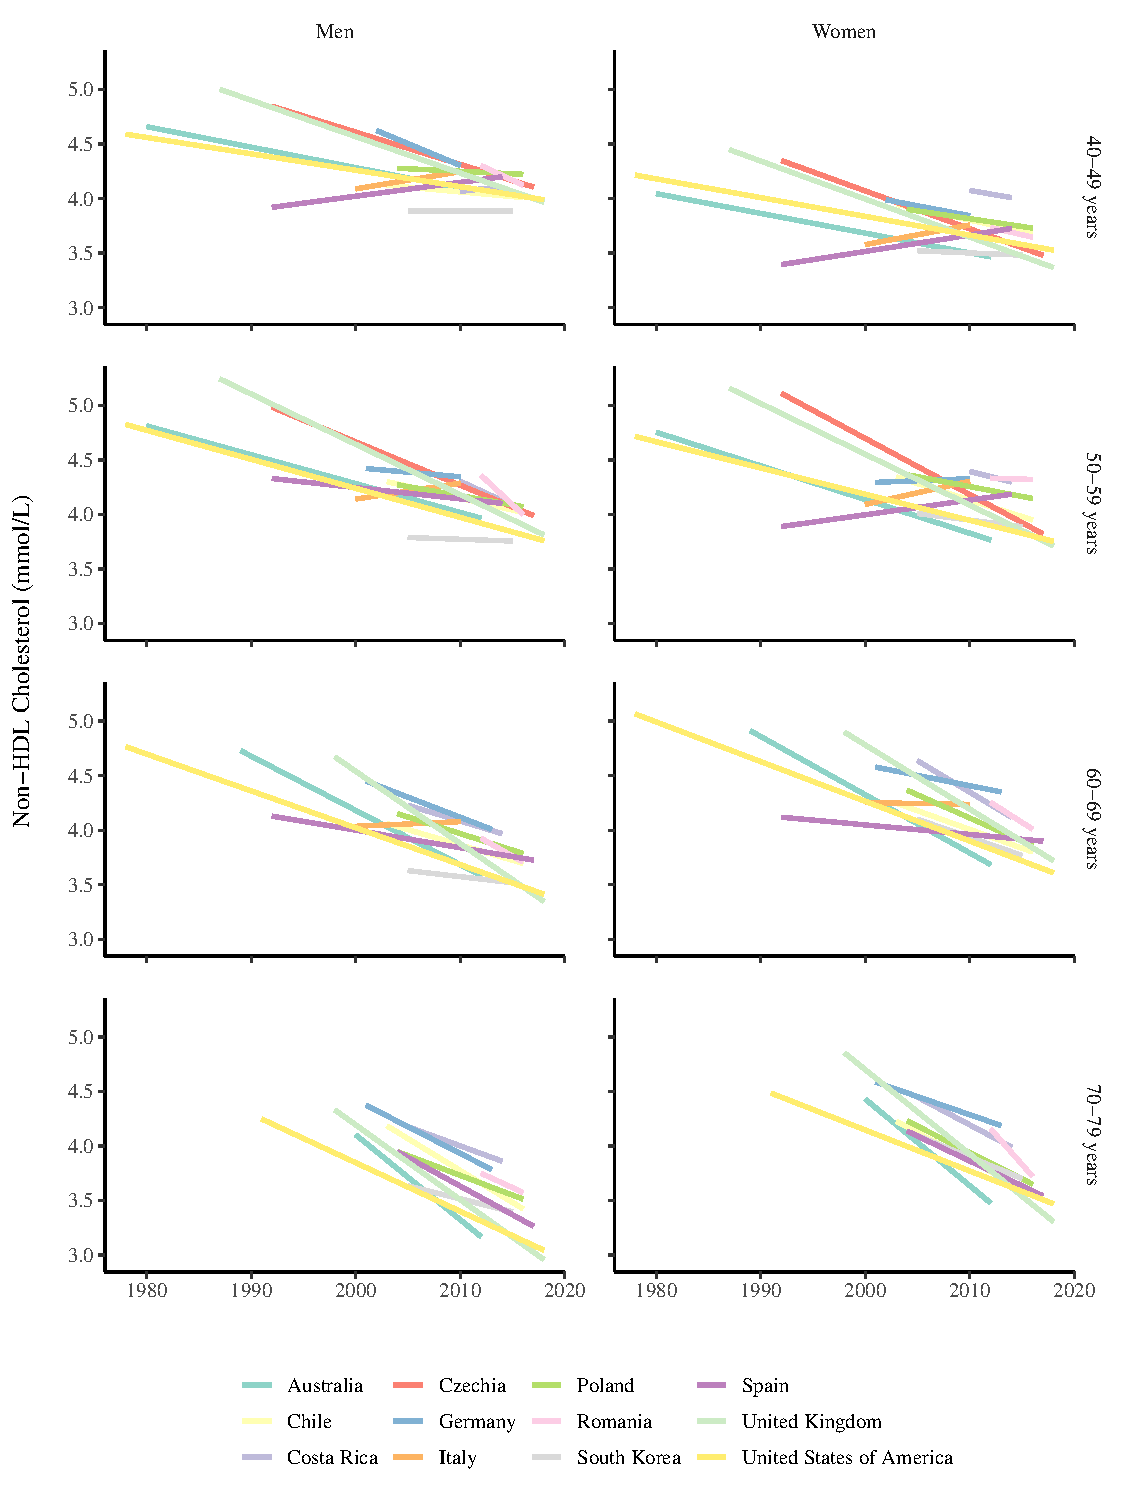
\includegraphics[width=0.9\linewidth]{../3_figures/figS_mean_chol_trends.pdf}
        \caption{Linear trends in mean Non-HDL-C level by country, age, and sex.}
        \label{fig:trends}
    \end{figure}
    \newpage 

    \begin{landscape}
        \subsection{Example distributional changes}

        \begin{figure}[H]
            \centering
            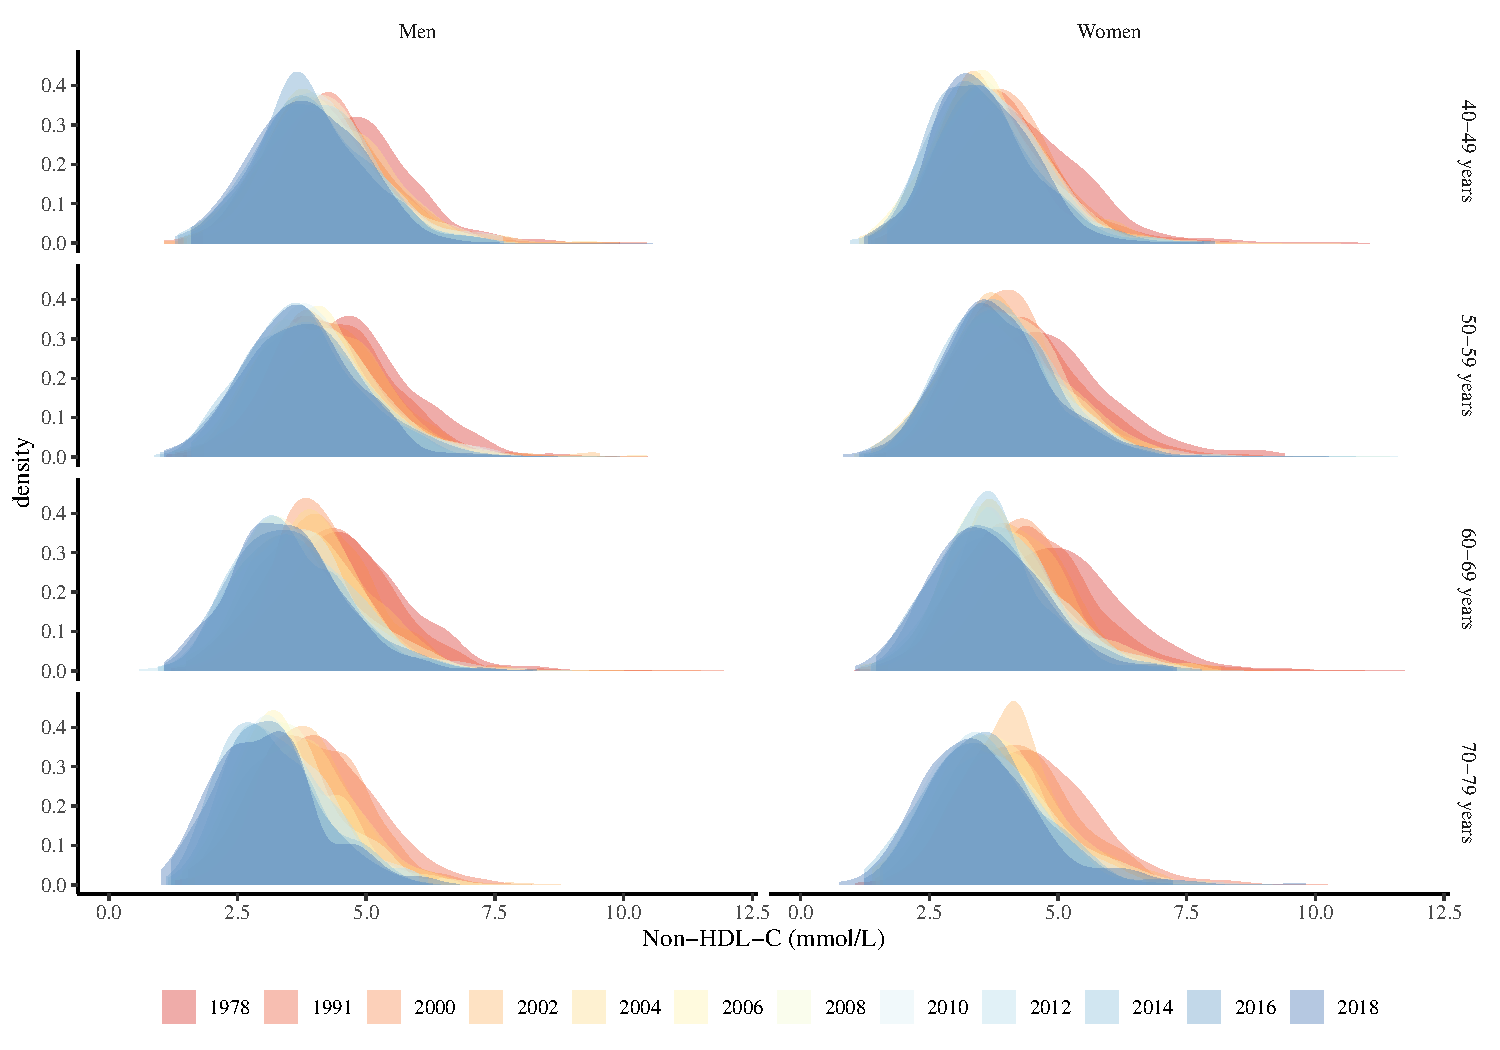
\includegraphics[width=\linewidth]{../3_figures/figS4_densities.pdf}
            \caption{Changes in distribution of Non-HDL-C in United States by sex and age group.}
            \label{fig:densities}
        \end{figure}

        \subsection{Country-by-country results}

        \begin{figure}[H]
            \centering
            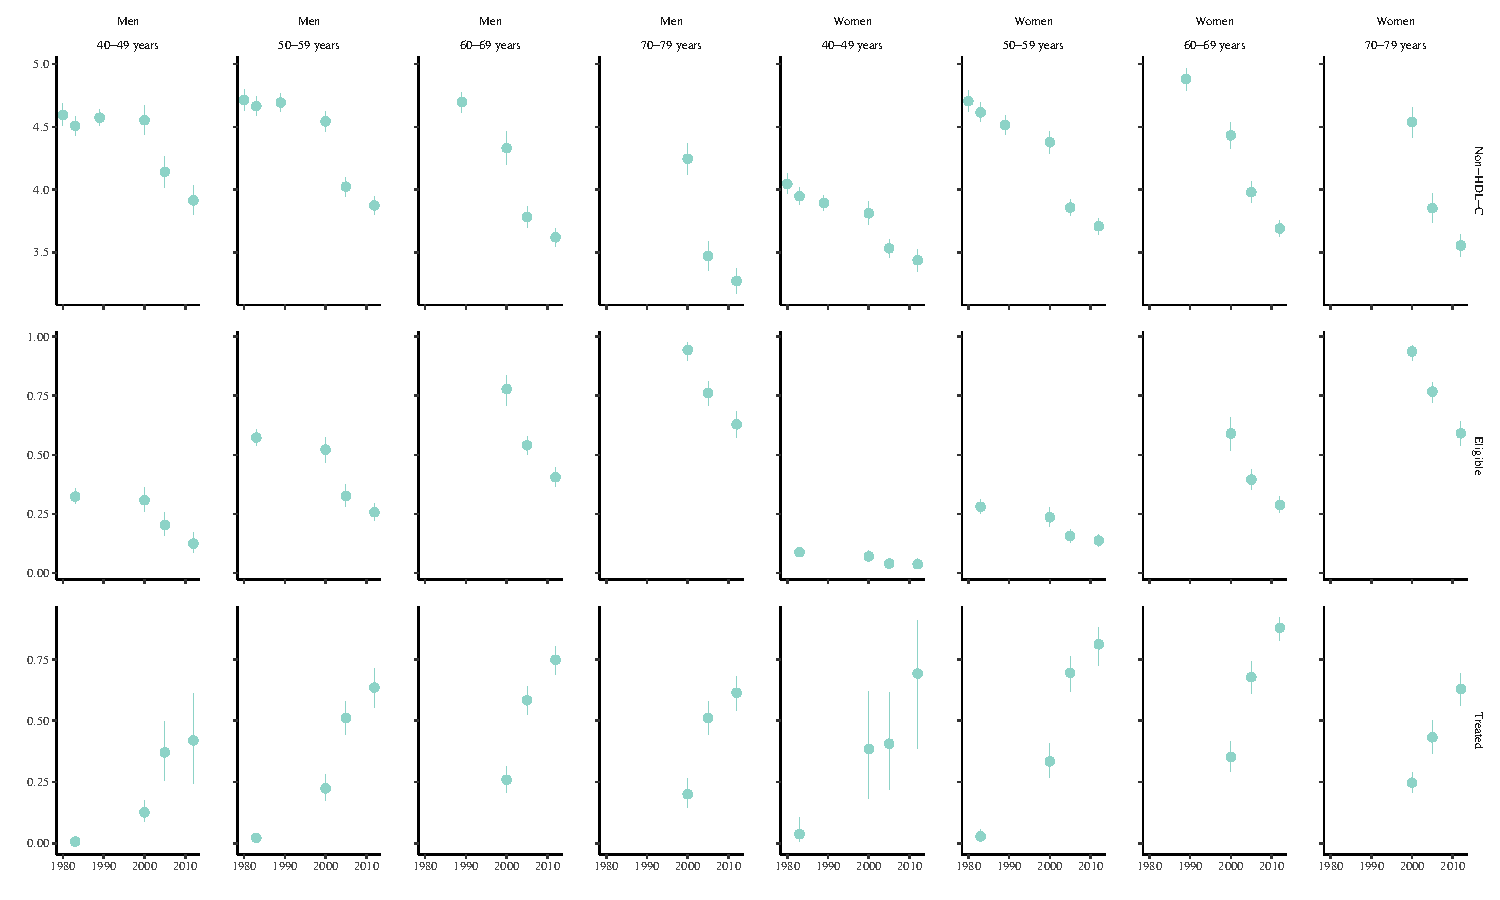
\includegraphics[width=\linewidth]{../3_figures/countries/fig_australia.pdf}
            \caption{Australia}
            \label{fig:australia}
        \end{figure}
    
        \begin{figure}[H]
            \centering
            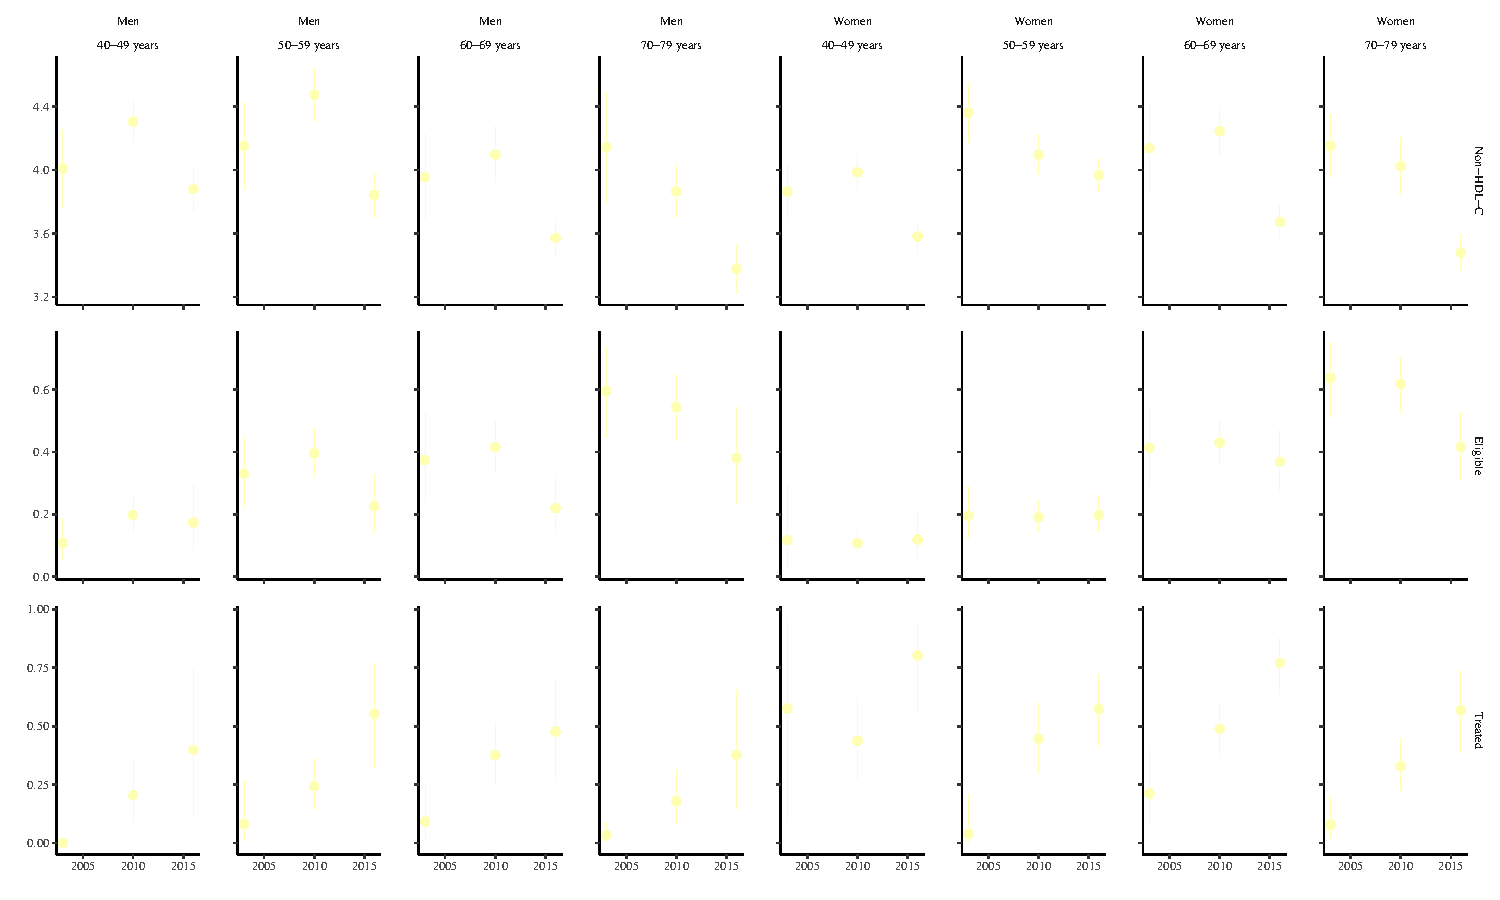
\includegraphics[width=\linewidth]{../3_figures/countries/fig_chile.pdf}
            \caption{Chile}
            \label{fig:chile}
        \end{figure}
    
        \begin{figure}[H]
            \centering
            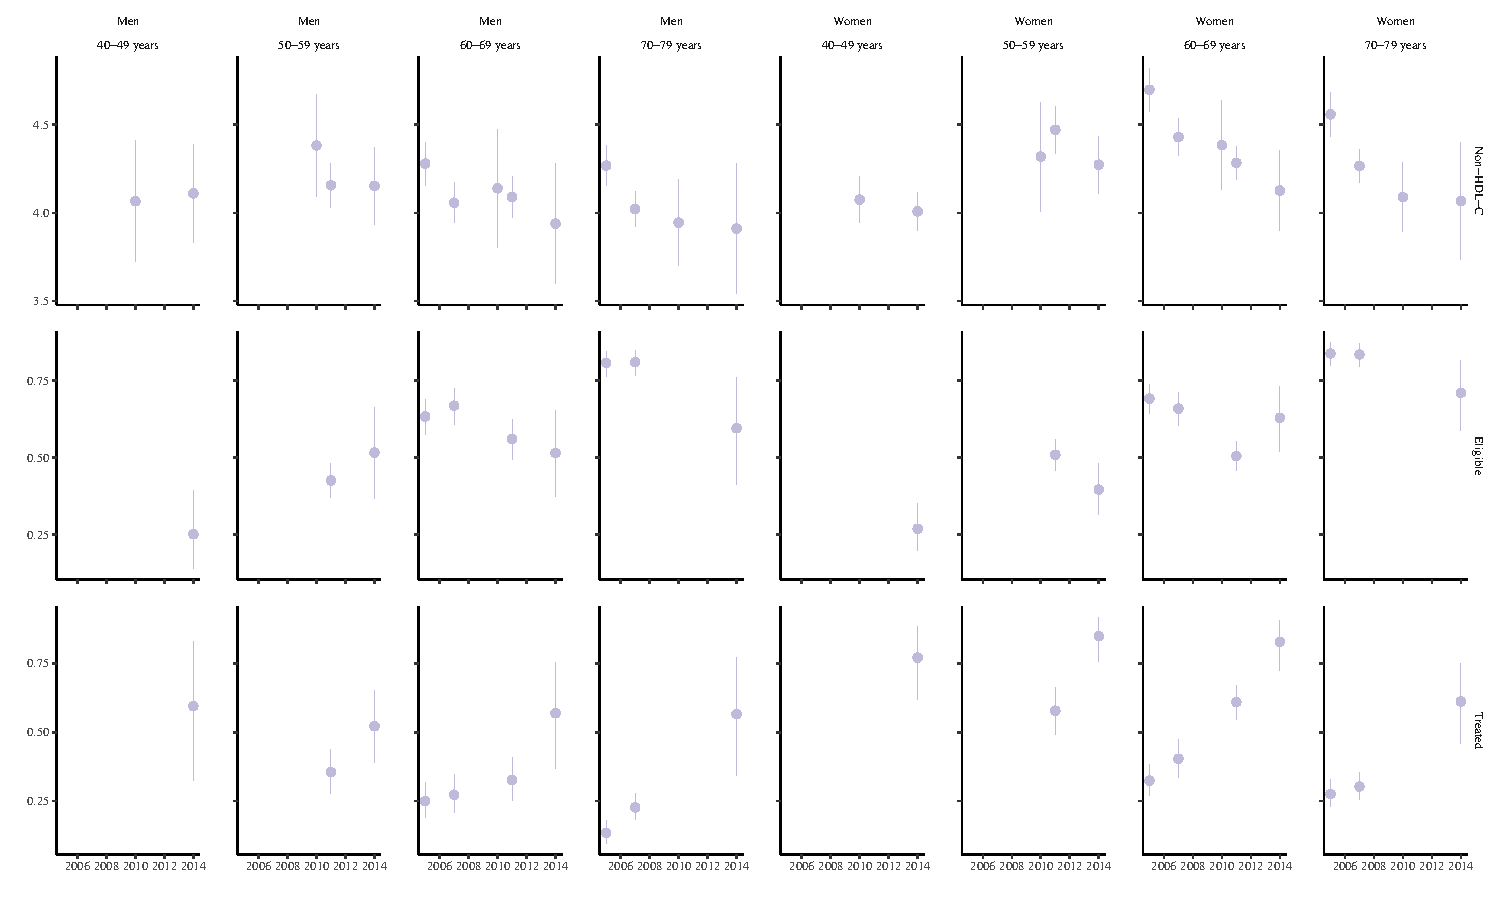
\includegraphics[width=\linewidth]{../3_figures/countries/fig_costa rica.pdf}
            \caption{Costa Rica}
            \label{fig:costa_rica}
        \end{figure}
    
        \begin{figure}[H]
            \centering
            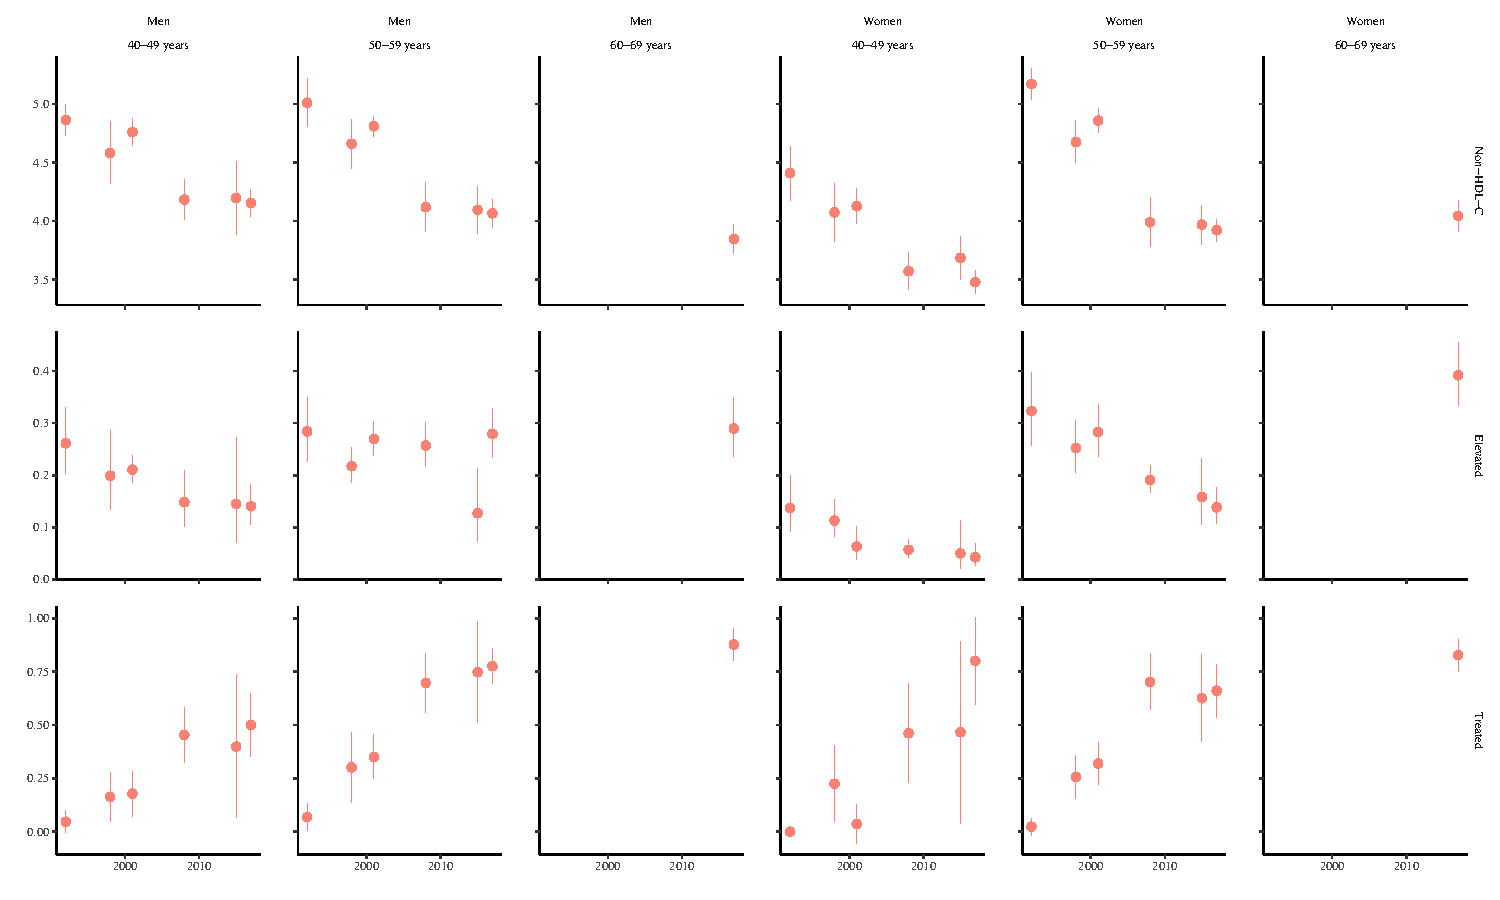
\includegraphics[width=\linewidth]{../3_figures/countries/fig_czechia.pdf}
            \caption{Czechia}
            \label{fig:czechia}
        \end{figure}

        \begin{figure}[H]
            \centering
            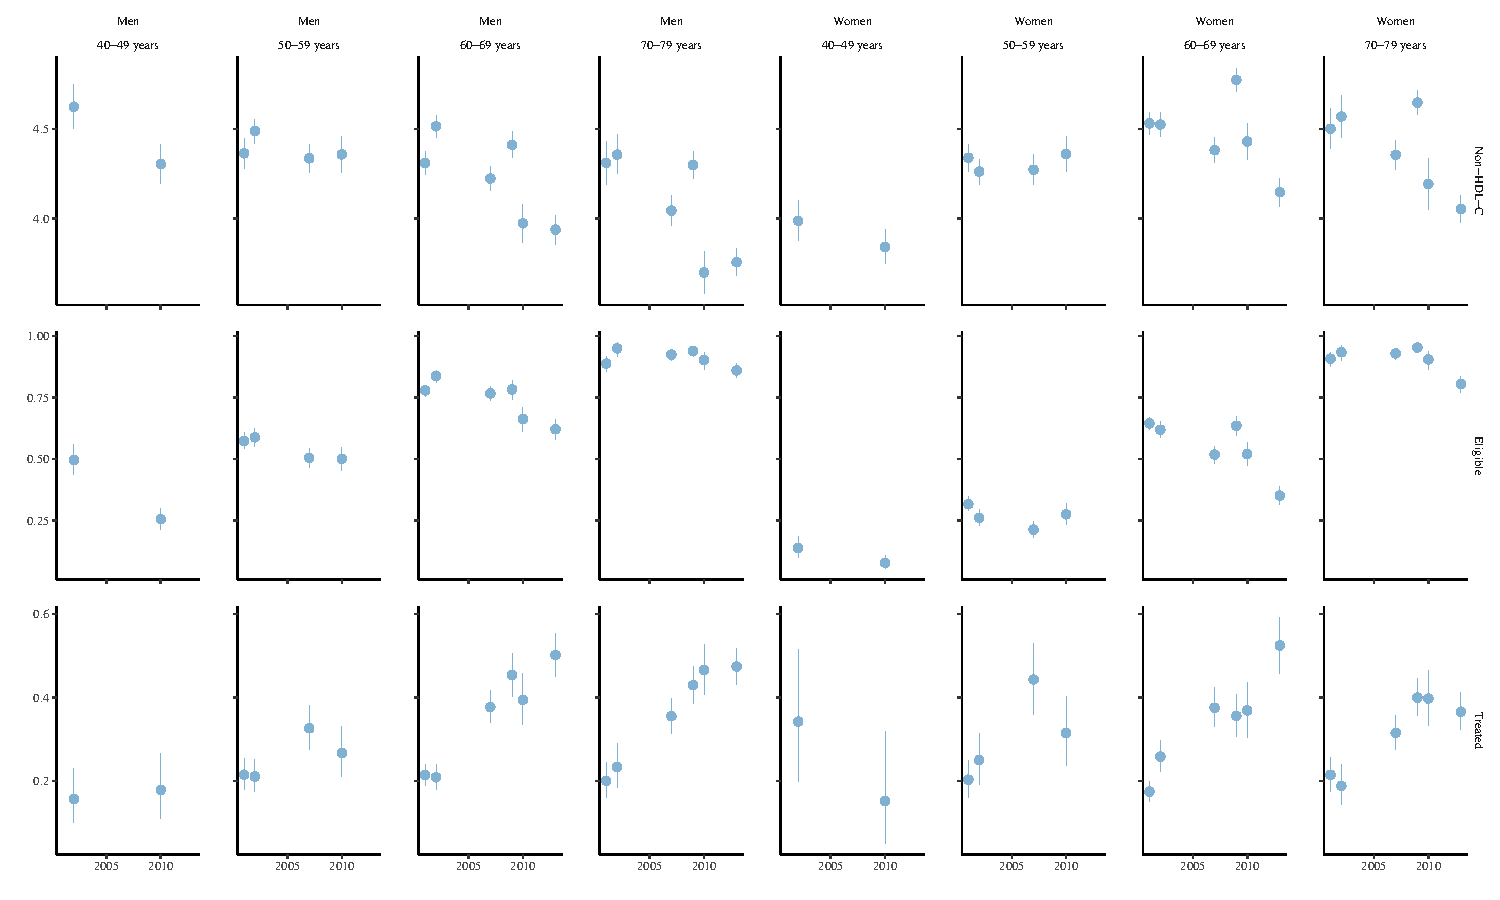
\includegraphics[width=\linewidth]{../3_figures/countries/fig_germany.pdf}
            \caption{Germany}
            \label{fig:germany}
        \end{figure}

        \begin{figure}[H]
            \centering
            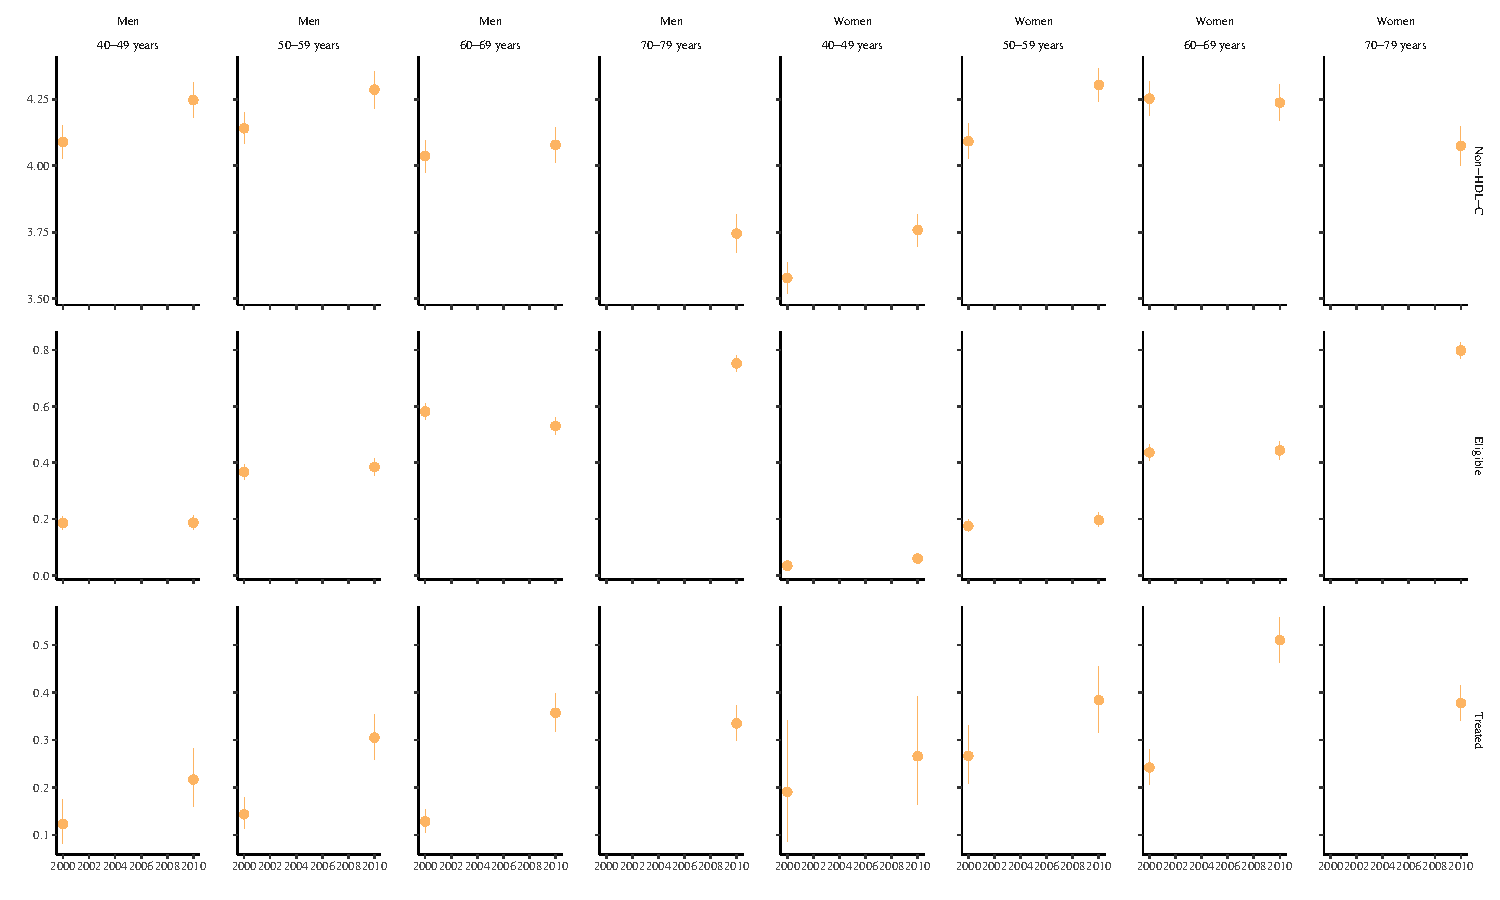
\includegraphics[width=\linewidth]{../3_figures/countries/fig_italy.pdf}
            \caption{Italy}
            \label{fig:italy}
        \end{figure}

        \begin{figure}[H]
            \centering
            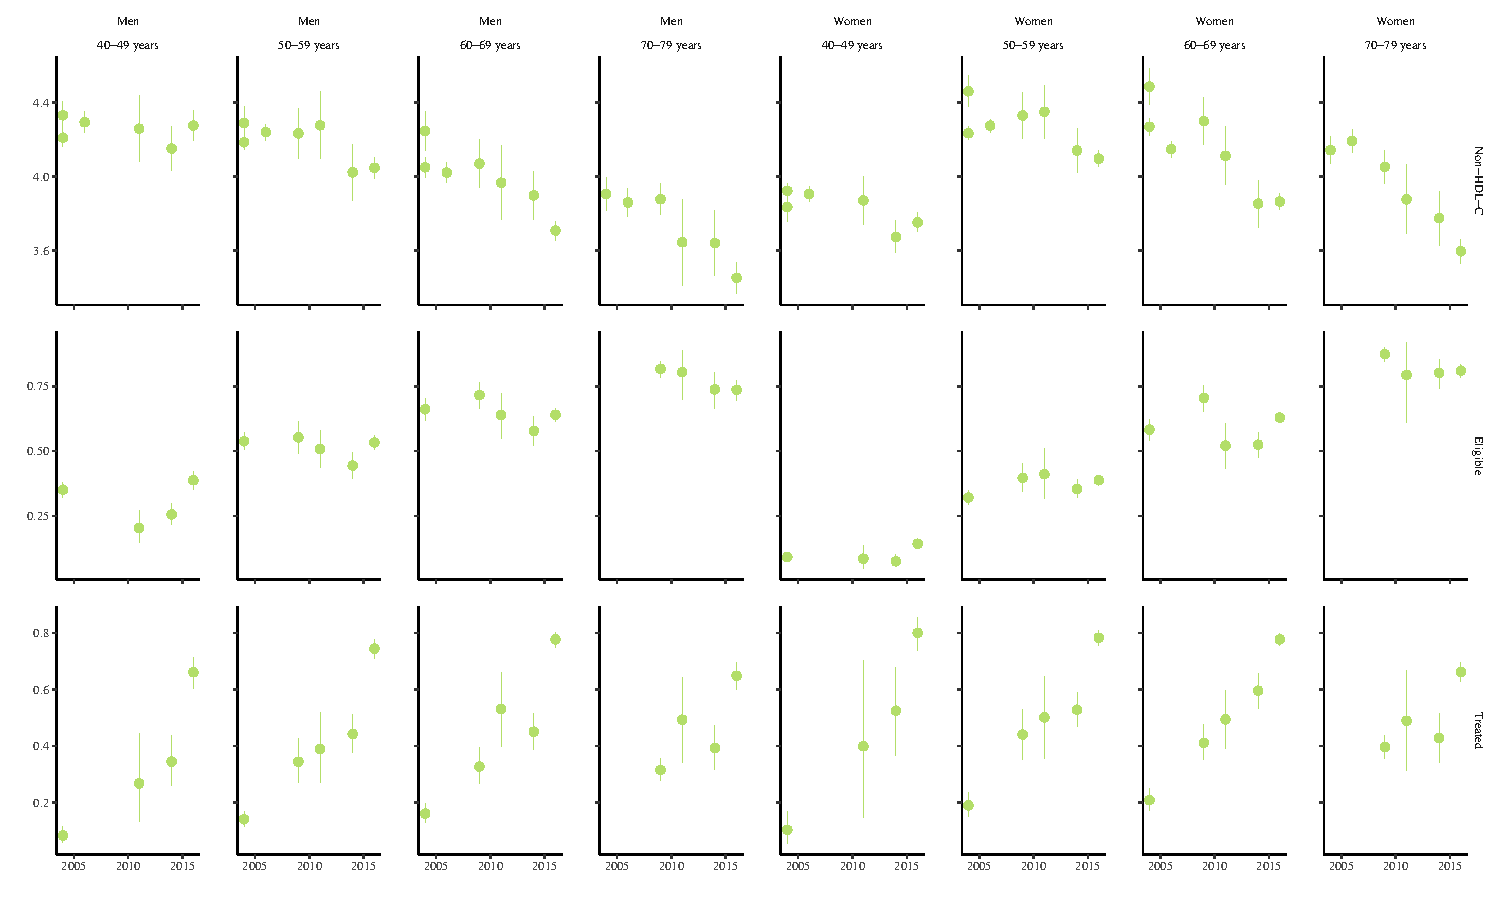
\includegraphics[width=\linewidth]{../3_figures/countries/fig_poland.pdf}
            \caption{Poland}
            \label{fig:poland}
        \end{figure}

        \begin{figure}[H]
            \centering
            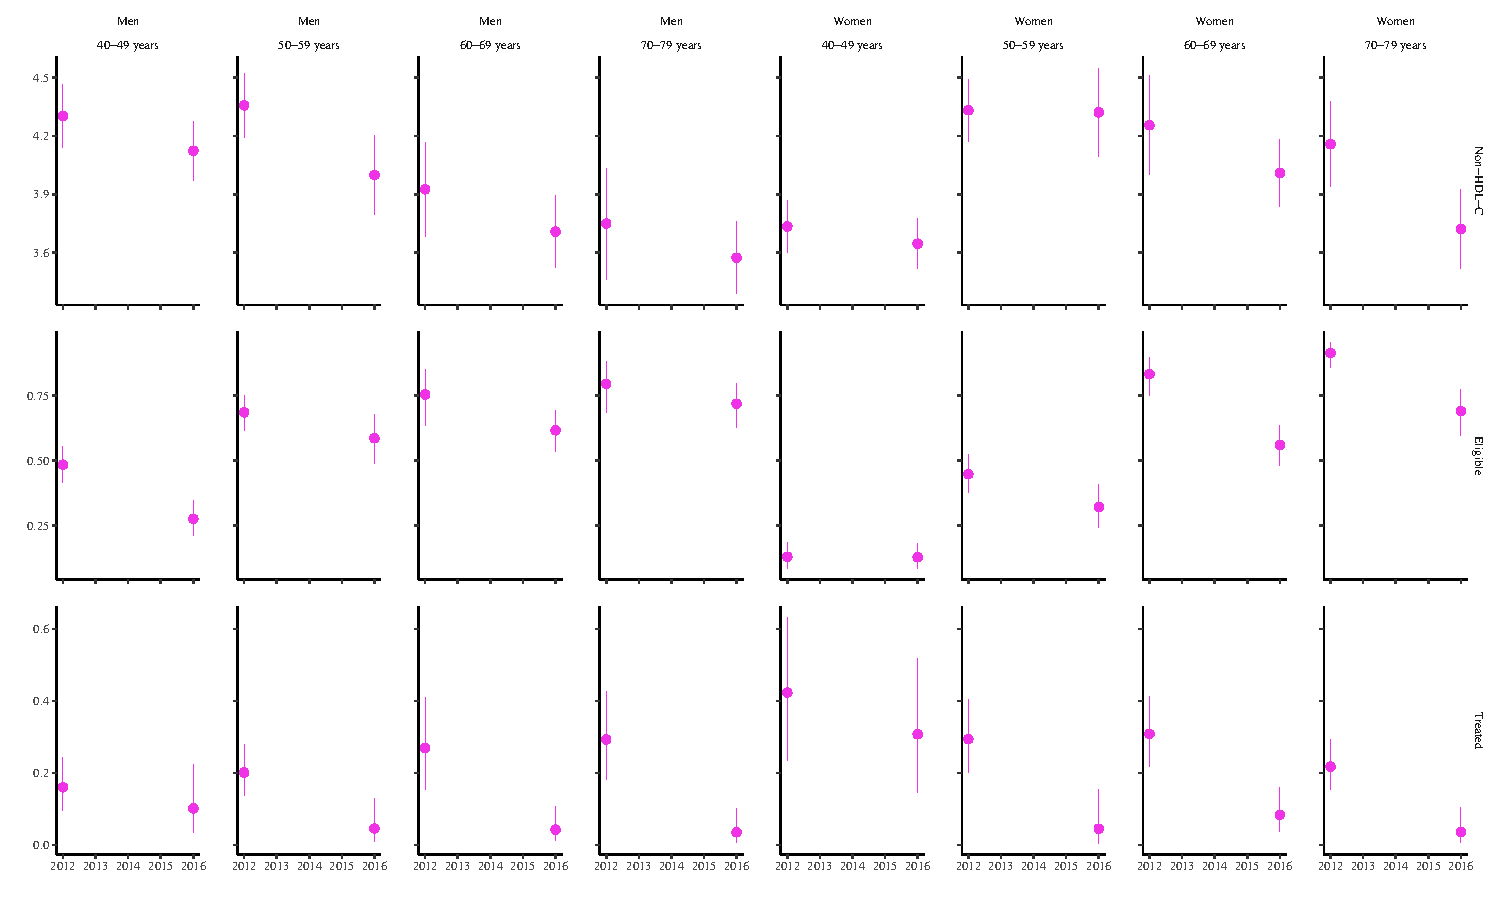
\includegraphics[width=\linewidth]{../3_figures/countries/fig_romania.pdf}
            \caption{Romania}
            \label{fig:romania}
        \end{figure}

        \begin{figure}[H]
            \centering
            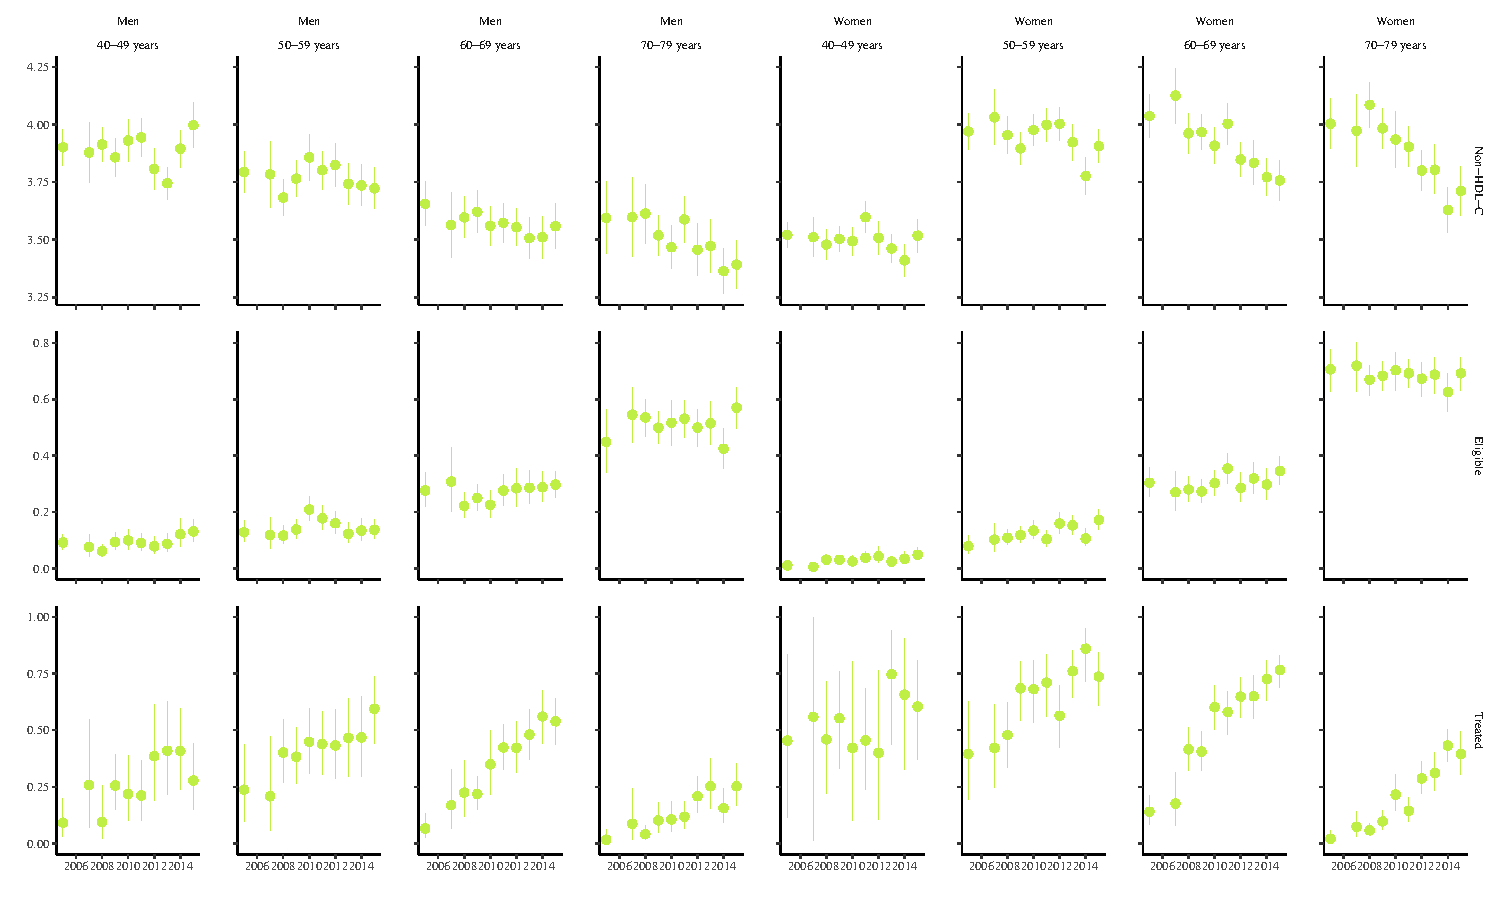
\includegraphics[width=\linewidth]{../3_figures/countries/fig_south korea.pdf}
            \caption{South Korea}
            \label{fig:korea}
        \end{figure}

        \begin{figure}[H]
            \centering
            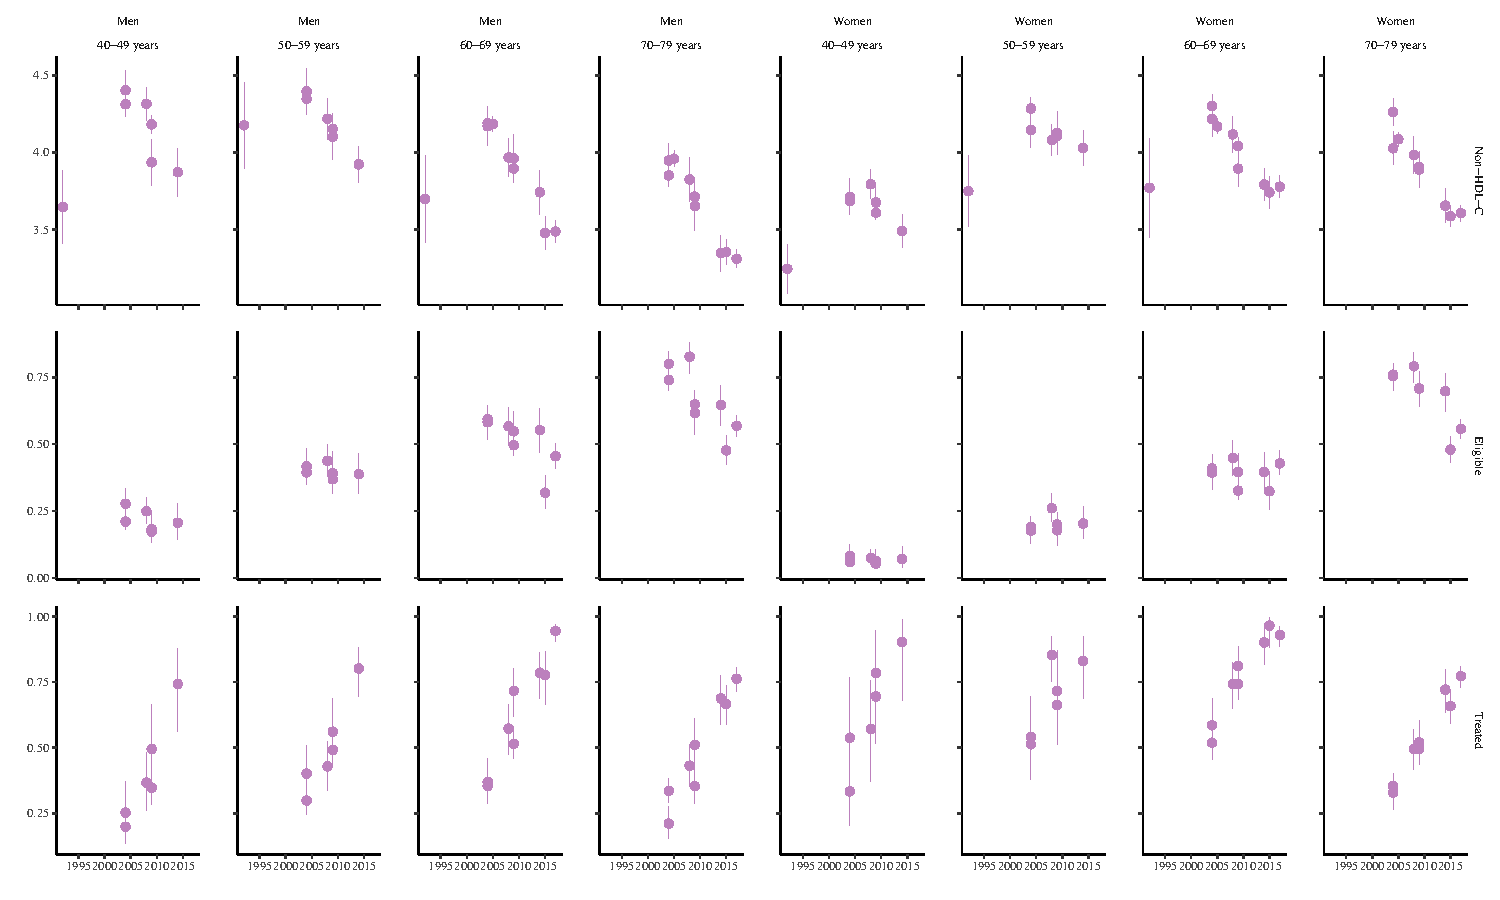
\includegraphics[width=\linewidth]{../3_figures/countries/fig_spain.pdf}
            \caption{Spain}
            \label{fig:spain}
        \end{figure}

        \begin{figure}[H]
            \centering
            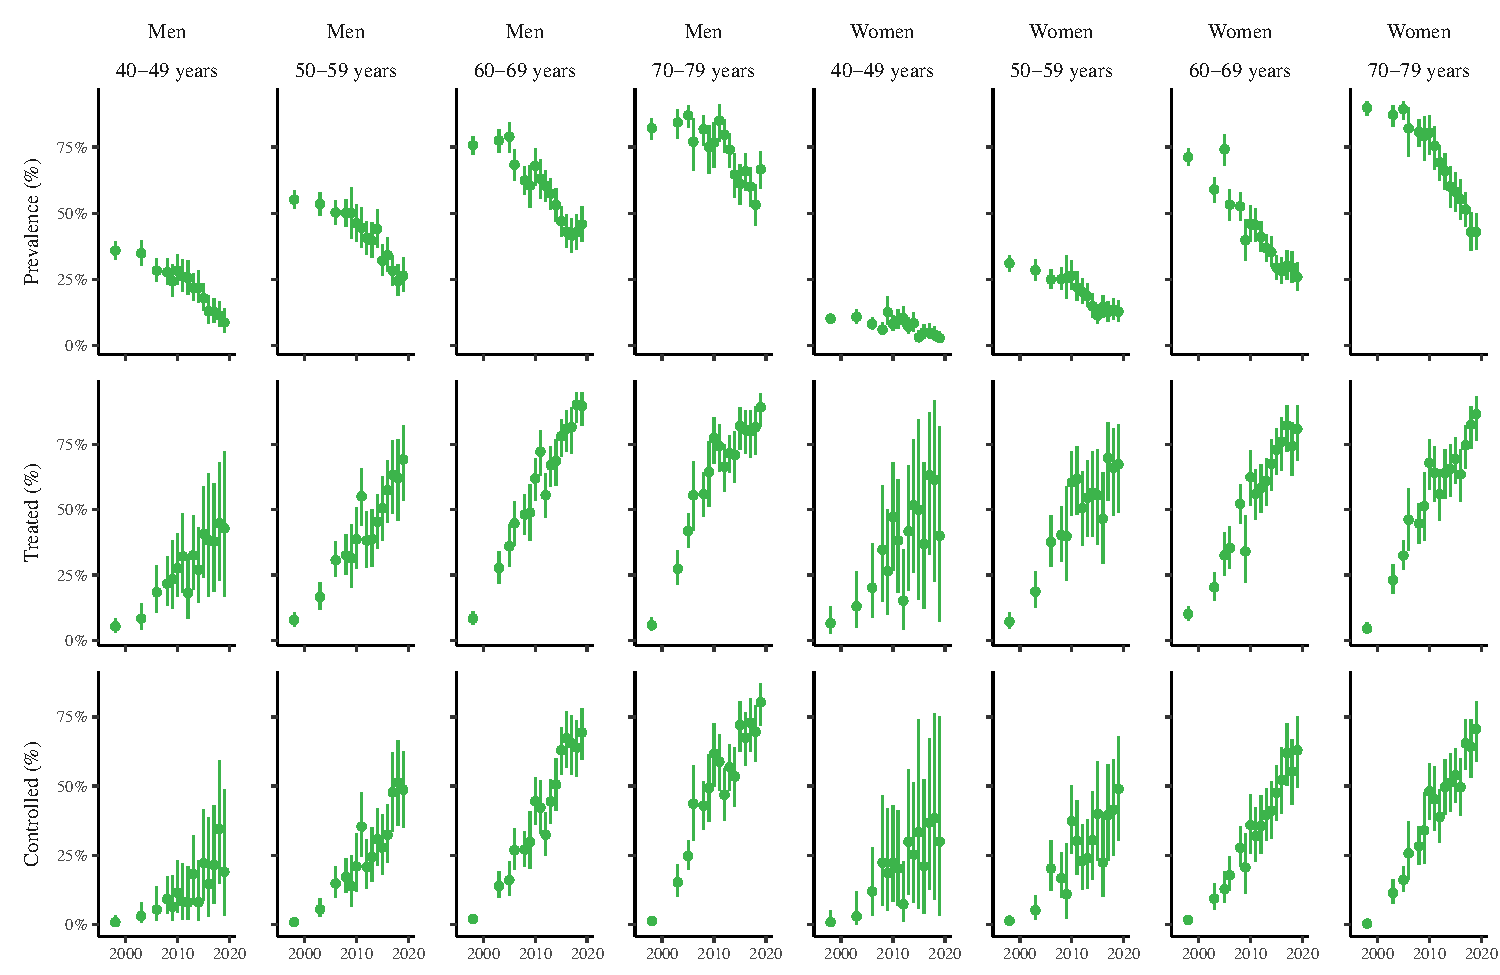
\includegraphics[width=\linewidth]{../3_figures/countries/fig_united kingdom.pdf}
            \caption{United Kingdom}
            \label{fig:uk}
        \end{figure}

        \begin{figure}[H]
            \centering
            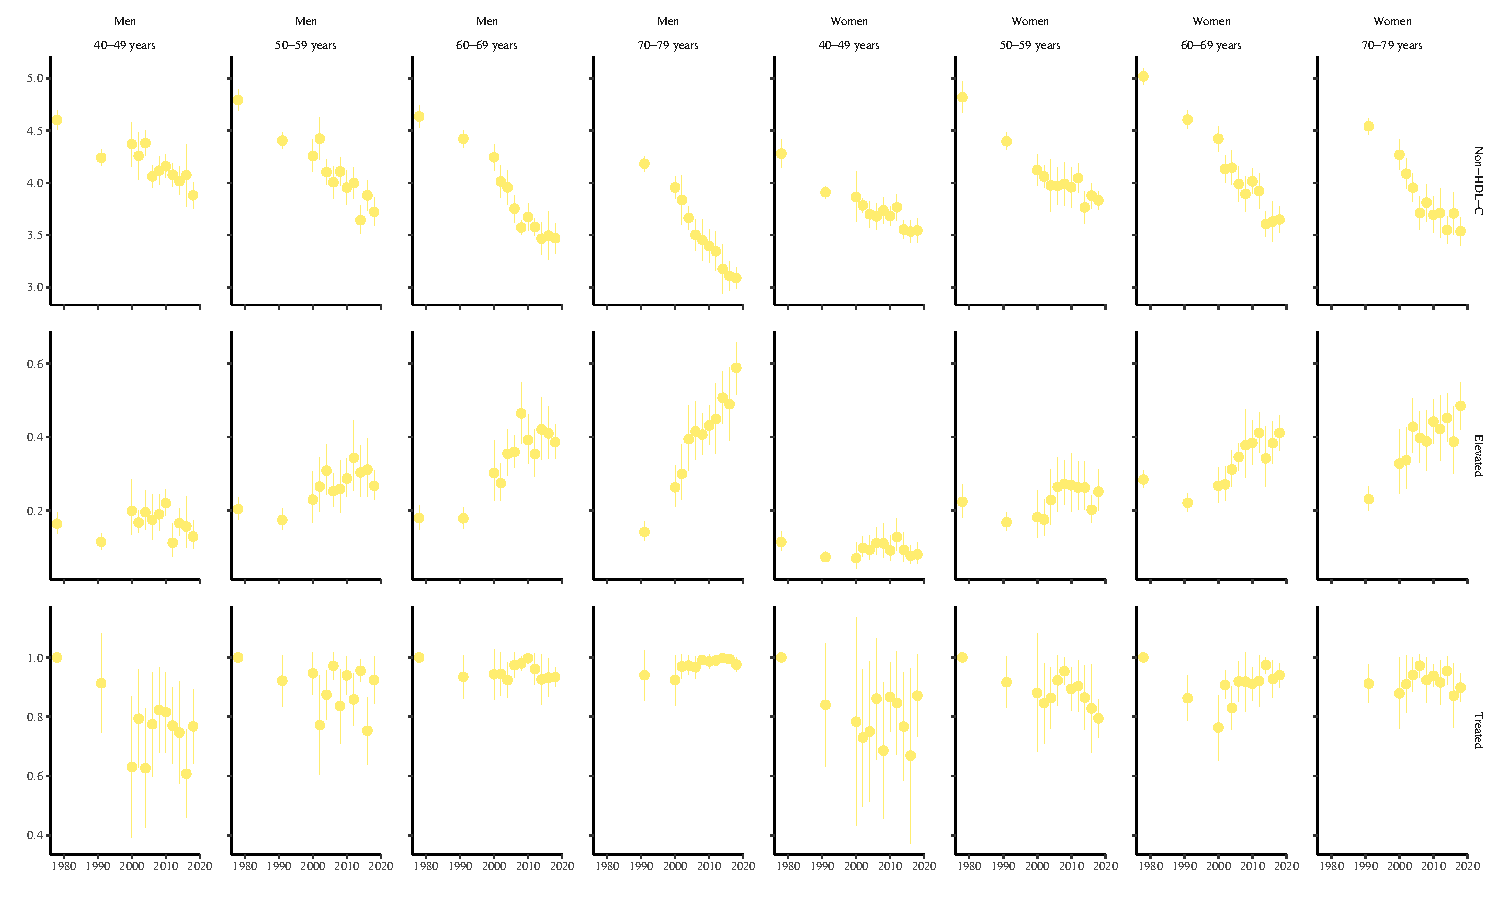
\includegraphics[width=\linewidth]{../3_figures/countries/fig_united states of america.pdf}
            \caption{United States of America}
            \label{fig:usa}
        \end{figure}
    \end{landscape}

    % \subsection{Missing cholesterol data}
    % \begin{singlespace}
    %     \begingroup\fontsize{7}{9}\selectfont

\begin{longtable}{llrllrr}
\toprule
\multicolumn{3}{c}{ } & \multicolumn{2}{c}{Missing} & \multicolumn{2}{c}{Mean} \\
\cmidrule(l{3pt}r{3pt}){4-5} \cmidrule(l{3pt}r{3pt}){6-7}
Country & Study ID & N & self\_chol, N (\%) & drug\_chol, N (\%) & self\_chol & drug\_chol\\
\midrule
\endfirsthead
\multicolumn{7}{@{}l}{\textit{(continued)}}\\
\toprule
Country & Study ID & N & self\_chol, N (\%) & drug\_chol, N (\%) & self\_chol & drug\_chol\\
\midrule
\endhead

\endfoot
\bottomrule
\endlastfoot
Australia & AUS\_1980\_RFPS & 2608 & 2608 (100.00\%) & 0 (0.00\%) & NaN & 0.02\\
Australia & AUS\_1983\_RFPS & 3509 & 3509 (100.00\%) & 0 (0.00\%) & NaN & 0.01\\
Australia & AUS\_1989\_RFPS & 5132 & 5132 (100.00\%) & 0 (0.00\%) & NaN & 0.04\\
Australia & AUS\_2000\_AusDiab & 8387 & 74 (0.88\%) & 76 (0.91\%) & 0.31 & 0.11\\
Australia & AUS\_2005\_AusDiab & 5467 & 87 (1.59\%) & 51 (0.93\%) & 0.39 & 0.18\\
Australia & AUS\_2012\_AusDiab & 4212 & 114 (2.71\%) & 2440 (57.93\%) & 0.43 & 0.48\\
\addlinespace
Chile & CHL\_2003\_ENS & 1242 & 1242 (100.00\%) & 0 (0.00\%) & NaN & 0.03\\
Chile & CHL\_2010\_ENS & 1560 & 1560 (100.00\%) & 17 (1.09\%) & NaN & 0.11\\
Chile & CHL\_2016\_ENS & 2261 & 2261 (100.00\%) & 0 (0.00\%) & NaN & 0.14\\
\addlinespace
Costa Rica & CRI\_2005\_CRELES & 1685 & 19 (1.13\%) & 0 (0.00\%) & 0.41 & 0.18\\
Costa Rica & CRI\_2007\_CRELES & 1380 & 4 (0.29\%) & 0 (0.00\%) & 0.54 & 0.22\\
Costa Rica & CRI\_2010\_CRFS & 1625 & 1625 (100.00\%) & 15 (0.92\%) & NaN & 0.30\\
Costa Rica & CRI\_2011\_CRELES & 2615 & 40 (1.53\%) & 46 (1.76\%) & 0.48 & 0.26\\
Costa Rica & CRI\_2014\_CRFS & 1300 & 1300 (100.00\%) & 9 (0.69\%) & NaN & 0.33\\
\addlinespace
Czechia & CZE\_1992\_MONICA & 1210 & 1210 (100.00\%) & 5 (0.41\%) & NaN & 0.01\\
Czechia & CZE\_1998\_postMONICA & 1881 & 1881 (100.00\%) & 12 (0.64\%) & NaN & 0.05\\
Czechia & CZE\_2001\_postMONICA & 1881 & 1881 (100.00\%) & 4 (0.21\%) & NaN & 0.06\\
Czechia & CZE\_2008\_postMONICA & 1925 & 1925 (100.00\%) & 3 (0.16\%) & NaN & 0.11\\
Czechia & CZE\_2015\_EHES & 524 & 524 (100.00\%) & 0 (0.00\%) & NaN & 0.07\\
Czechia & CZE\_2017\_MONICA & 1934 & 1934 (100.00\%) & 35 (1.81\%) & NaN & 0.15\\
\addlinespace
Germany & DEU\_2001\_ESTHER & 6003 & 6003 (100.00\%) & 1 (0.02\%) & NaN & 0.13\\
Germany & DEU\_2002\_HNRS & 4779 & 4779 (100.00\%) & 308 (6.44\%) & NaN & 0.13\\
Germany & DEU\_2007\_HNRS & 4111 & 4111 (100.00\%) & 0 (0.00\%) & NaN & 0.22\\
Germany & DEU\_2009\_ESTHER & 4067 & 4067 (100.00\%) & 30 (0.74\%) & NaN & 0.34\\
Germany & DEU\_2010\_SHIPTREND & 3256 & 3256 (100.00\%) & 3256 (100.00\%) & NaN & NaN\\
Germany & DEU\_2013\_HNRS & 2435 & 2435 (100.00\%) & 0 (0.00\%) & NaN & 0.30\\
\addlinespace
Italy & ITA\_2000\_OEC & 7361 & 7361 (100.00\%) & 1 (0.01\%) & NaN & 0.05\\
Italy & ITA\_2010\_OEC & 7837 & 7837 (100.00\%) & 73 (0.93\%) & NaN & 0.15\\
\addlinespace
Poland & POL\_2004\_LIPIDOGRAM & 15133 & 0 (0.00\%) & 0 (0.00\%) & 0.53 & 0.32\\
Poland & POL\_2004\_WOBASZ & 7490 & 7490 (100.00\%) & 5377 (71.79\%) & NaN & 0.21\\
Poland & POL\_2006\_LIPIDOGRAM & 15796 & 0 (0.00\%) & 0 (0.00\%) & 0.52 & 0.34\\
Poland & POL\_2009\_PolSenior & 2821 & 2821 (100.00\%) & 2821 (100.00\%) & NaN & NaN\\
Poland & POL\_2011\_NATPOL & 1407 & 1407 (100.00\%) & 0 (0.00\%) & NaN & 0.20\\
Poland & POL\_2014\_WOBASZ & 3842 & 185 (4.82\%) & 200 (5.21\%) & 0.43 & 0.20\\
Poland & POL\_2016\_LIPIDOGRAM & 11423 & 11423 (100.00\%) & 0 (0.00\%) & NaN & 0.38\\
\addlinespace
Romania & ROU\_2012\_SEPHAR & 1237 & 1237 (100.00\%) & 1237 (100.00\%) & NaN & NaN\\
Romania & ROU\_2016\_SEPHAR & 1275 & 1275 (100.00\%) & 1275 (100.00\%) & NaN & NaN\\
\addlinespace
South Korea & KOR\_2005\_KNHANES & 3366 & 3366 (100.00\%) & 10 (0.30\%) & NaN & 0.02\\
South Korea & KOR\_2007\_KNHANES & 1772 & 1772 (100.00\%) & 33 (1.86\%) & NaN & 0.03\\
South Korea & KOR\_2008\_KNHANES & 4051 & 4051 (100.00\%) & 28 (0.69\%) & NaN & 0.04\\
South Korea & KOR\_2009\_KNHANES & 4515 & 4515 (100.00\%) & 16 (0.35\%) & NaN & 0.06\\
South Korea & KOR\_2010\_KNHANES & 3815 & 3815 (100.00\%) & 43 (1.13\%) & NaN & 0.08\\
South Korea & KOR\_2011\_KNHANES & 3922 & 3922 (100.00\%) & 77 (1.96\%) & NaN & 0.09\\
South Korea & KOR\_2012\_KNHANES & 3775 & 3775 (100.00\%) & 188 (4.98\%) & NaN & 0.10\\
South Korea & KOR\_2013\_KNHANES & 3444 & 3444 (100.00\%) & 188 (5.46\%) & NaN & 0.11\\
South Korea & KOR\_2014\_KNHANES & 3386 & 3386 (100.00\%) & 286 (8.45\%) & NaN & 0.12\\
South Korea & KOR\_2015\_KNHANES & 3587 & 3587 (100.00\%) & 206 (5.74\%) & NaN & 0.14\\
\addlinespace
Spain & ESP\_1992\_CVDRF & 1157 & 1157 (100.00\%) & 2 (0.17\%) & NaN & 0.04\\
Spain & ESP\_2004\_RECCyL & 2359 & 2359 (100.00\%) & 39 (1.65\%) & NaN & 0.15\\
Spain & ESP\_2004\_REGICOR & 5643 & 5643 (100.00\%) & 159 (2.82\%) & NaN & 0.14\\
Spain & ESP\_2005\_PREVICTUS & 5585 & 5585 (100.00\%) & 270 (4.83\%) & NaN & 0.44\\
Spain & ESP\_2008\_HERMEX & 2084 & 2084 (100.00\%) & 0 (0.00\%) & NaN & 0.22\\
Spain & ESP\_2009\_ENRICA & 8176 & 8176 (100.00\%) & 5378 (65.78\%) & NaN & 0.46\\
Spain & ESP\_2009\_RECCyL & 1875 & 1875 (100.00\%) & 43 (2.29\%) & NaN & 0.24\\
Spain & ESP\_2014\_RECCyL & 1803 & 1803 (100.00\%) & 55 (3.05\%) & NaN & 0.30\\
Spain & ESP\_2015\_ENRICA & 1217 & 0 (0.00\%) & 0 (0.00\%) & 0.53 & 0.30\\
Spain & ESP\_2017\_ENRICASenior & 2438 & 2438 (100.00\%) & 2438 (100.00\%) & NaN & NaN\\
\addlinespace
United Kingdom & GBR\_1987\_DNS & 764 & 764 (100.00\%) & 213 (27.88\%) & NaN & 0.00\\
United Kingdom & GBR\_1998\_HSE & 6274 & 6274 (100.00\%) & 0 (0.00\%) & NaN & 0.04\\
United Kingdom & GBR\_2000\_HSE & 157 & 157 (100.00\%) & 0 (0.00\%) & NaN & 0.03\\
United Kingdom & GBR\_2003\_HSE & 5276 & 5276 (100.00\%) & 0 (0.00\%) & NaN & 0.10\\
United Kingdom & GBR\_2005\_HSE & 1761 & 1761 (100.00\%) & 0 (0.00\%) & NaN & 0.29\\
United Kingdom & GBR\_2006\_HSE & 4940 & 4940 (100.00\%) & 0 (0.00\%) & NaN & 0.16\\
United Kingdom & GBR\_2008\_HSE & 4861 & 4861 (100.00\%) & 0 (0.00\%) & NaN & 0.18\\
United Kingdom & GBR\_2009\_HSE & 1549 & 1549 (100.00\%) & 0 (0.00\%) & NaN & 0.17\\
United Kingdom & GBR\_2010\_HSE & 2582 & 2582 (100.00\%) & 352 (13.63\%) & NaN & 0.23\\
United Kingdom & GBR\_2010\_NDNS & 1144 & 1144 (100.00\%) & 467 (40.82\%) & NaN & 0.32\\
United Kingdom & GBR\_2011\_HSE & 2634 & 2634 (100.00\%) & 388 (14.73\%) & NaN & 0.23\\
United Kingdom & GBR\_2012\_HSE & 2725 & 2725 (100.00\%) & 0 (0.00\%) & NaN & 0.20\\
United Kingdom & GBR\_2013\_HSE & 3050 & 3050 (100.00\%) & 0 (0.00\%) & NaN & 0.21\\
United Kingdom & GBR\_2014\_HSE & 2651 & 2651 (100.00\%) & 0 (0.00\%) & NaN & 0.20\\
United Kingdom & GBR\_2014\_NDNS & 485 & 485 (100.00\%) & 0 (0.00\%) & NaN & 0.20\\
United Kingdom & GBR\_2015\_HSE & 2694 & 2694 (100.00\%) & 0 (0.00\%) & NaN & 0.21\\
United Kingdom & GBR\_2016\_HSE & 2624 & 2624 (100.00\%) & 0 (0.00\%) & NaN & 0.21\\
United Kingdom & GBR\_2016\_NDNS & 463 & 463 (100.00\%) & 0 (0.00\%) & NaN & 0.18\\
United Kingdom & GBR\_2017\_HSE & 2697 & 2697 (100.00\%) & 0 (0.00\%) & NaN & 0.21\\
United Kingdom & GBR\_2017\_NDNS & 210 & 210 (100.00\%) & 0 (0.00\%) & NaN & 0.16\\
United Kingdom & GBR\_2018\_HSE & 2445 & 2445 (100.00\%) & 0 (0.00\%) & NaN & 0.20\\
\addlinespace
United States of America & USA\_1978\_NHANES & 5077 & 5077 (100.00\%) & 5038 (99.23\%) & NaN & 1.00\\
United States of America & USA\_1991\_NHANES & 8167 & 8167 (100.00\%) & 7576 (92.76\%) & NaN & 0.74\\
United States of America & USA\_2000\_NHANES & 2364 & 2364 (100.00\%) & 942 (39.85\%) & NaN & 0.23\\
United States of America & USA\_2002\_NHANES & 2617 & 2617 (100.00\%) & 953 (36.42\%) & NaN & 0.24\\
United States of America & USA\_2004\_NHANES & 2511 & 2511 (100.00\%) & 834 (33.21\%) & NaN & 0.32\\
United States of America & USA\_2006\_NHANES & 2453 & 2453 (100.00\%) & 800 (32.61\%) & NaN & 0.32\\
United States of America & USA\_2008\_NHANES & 3049 & 3049 (100.00\%) & 905 (29.68\%) & NaN & 0.36\\
United States of America & USA\_2010\_NHANES & 3421 & 3421 (100.00\%) & 1014 (29.64\%) & NaN & 0.36\\
United States of America & USA\_2012\_NHANES & 2875 & 2875 (100.00\%) & 420 (14.61\%) & NaN & 0.28\\
United States of America & USA\_2014\_NHANES & 3223 & 3223 (100.00\%) & 518 (16.07\%) & NaN & 0.29\\
United States of America & USA\_2016\_NHANES & 3099 & 3099 (100.00\%) & 414 (13.36\%) & NaN & 0.28\\
United States of America & USA\_2018\_NHANES & 3102 & 0 (0.00\%) & 12 (0.39\%) & 0.45 & 0.29\\*
\end{longtable}
\endgroup{}

    %     \label{tab:missing_chol_data}
    % \end{singlespace}

    % \newpage
    
    % \subsection{Missing smoking data}
    % \begin{singlespace}
    %     \begingroup\fontsize{7}{9}\selectfont

\begin{longtable}{llrllrr}
\toprule
\multicolumn{3}{c}{ } & \multicolumn{2}{c}{Missing} & \multicolumn{2}{c}{Mean} \\
\cmidrule(l{3pt}r{3pt}){4-5} \cmidrule(l{3pt}r{3pt}){6-7}
Country & Study ID & N & smoke\_ever, N (\%) & smoker, N (\%) & smoke\_ever & smoker\\
\midrule
\endfirsthead
\multicolumn{7}{@{}l}{\textit{(continued)}}\\
\toprule
Country & Study ID & N & smoke\_ever, N (\%) & smoker, N (\%) & smoke\_ever & smoker\\
\midrule
\endhead

\endfoot
\bottomrule
\endlastfoot
Australia & AUS\_1980\_RFPS & 2608 & 0 (0.00\%) & 0 (0.00\%) & 0.55 & 0.32\\
Australia & AUS\_1983\_RFPS & 3509 & 0 (0.00\%) & 5 (0.14\%) & 0.53 & 0.29\\
Australia & AUS\_1989\_RFPS & 5132 & 0 (0.00\%) & 0 (0.00\%) & 0.48 & 0.20\\
Australia & AUS\_2000\_AusDiab & 8387 & 154 (1.84\%) & 154 (1.84\%) & 0.45 & 0.14\\
Australia & AUS\_2005\_AusDiab & 5467 & 253 (4.63\%) & 253 (4.63\%) & 0.43 & 0.09\\
Australia & AUS\_2012\_AusDiab & 4212 & 249 (5.91\%) & 249 (5.91\%) & 0.40 & 0.06\\
\addlinespace
Chile & CHL\_2003\_ENS & 1242 & 36 (2.90\%) & 24 (1.93\%) & 0.50 & 0.29\\
Chile & CHL\_2010\_ENS & 1560 & 18 (1.15\%) & 54 (3.46\%) & 0.49 & 0.30\\
Chile & CHL\_2016\_ENS & 2261 & 0 (0.00\%) & 0 (0.00\%) & 0.52 & 0.26\\
\addlinespace
Costa Rica & CRI\_2005\_CRELES & 1685 & 2 (0.12\%) & 2 (0.12\%) & 0.43 & 0.10\\
Costa Rica & CRI\_2007\_CRELES & 1380 & 1 (0.07\%) & 1 (0.07\%) & 0.43 & 0.09\\
Costa Rica & CRI\_2010\_CRFS & 1625 & 0 (0.00\%) & 0 (0.00\%) & 0.09 & 0.08\\
Costa Rica & CRI\_2011\_CRELES & 2615 & 1 (0.04\%) & 1 (0.04\%) & 0.37 & 0.11\\
Costa Rica & CRI\_2014\_CRFS & 1300 & 1300 (100.00\%) & 2 (0.15\%) & NaN & 0.08\\
\addlinespace
Czechia & CZE\_1992\_MONICA & 1210 & 1210 (100.00\%) & 0 (0.00\%) & NaN & 0.32\\
Czechia & CZE\_1998\_postMONICA & 1881 & 1 (0.05\%) & 1 (0.05\%) & 0.52 & 0.33\\
Czechia & CZE\_2001\_postMONICA & 1881 & 0 (0.00\%) & 0 (0.00\%) & 0.55 & 0.33\\
Czechia & CZE\_2008\_postMONICA & 1925 & 1 (0.05\%) & 1 (0.05\%) & 0.56 & 0.32\\
Czechia & CZE\_2015\_EHES & 524 & 0 (0.00\%) & 0 (0.00\%) & 0.52 & 0.31\\
Czechia & CZE\_2017\_MONICA & 1934 & 8 (0.41\%) & 8 (0.41\%) & 0.43 & 0.24\\
\addlinespace
Germany & DEU\_2001\_ESTHER & 6003 & 144 (2.40\%) & 144 (2.40\%) & 0.50 & 0.16\\
Germany & DEU\_2002\_HNRS & 4779 & 9 (0.19\%) & 9 (0.19\%) & 0.58 & 0.24\\
Germany & DEU\_2007\_HNRS & 4111 & 7 (0.17\%) & 7 (0.17\%) & 1.00 & 0.00\\
Germany & DEU\_2009\_ESTHER & 4067 & 21 (0.52\%) & 21 (0.52\%) & 0.44 & 0.08\\
Germany & DEU\_2010\_SHIPTREND & 3256 & 15 (0.46\%) & 15 (0.46\%) & 0.62 & 0.22\\
Germany & DEU\_2013\_HNRS & 2435 & 5 (0.21\%) & 5 (0.21\%) & 0.56 & 0.12\\
\addlinespace
Italy & ITA\_2000\_OEC & 7361 & 7361 (100.00\%) & 2 (0.03\%) & NaN & 0.28\\
Italy & ITA\_2010\_OEC & 7837 & 7837 (100.00\%) & 8 (0.10\%) & NaN & 0.20\\
\addlinespace
Poland & POL\_2004\_LIPIDOGRAM & 15133 & 15133 (100.00\%) & 0 (0.00\%) & NaN & 0.20\\
Poland & POL\_2004\_WOBASZ & 7490 & 137 (1.83\%) & 137 (1.83\%) & 0.59 & 0.33\\
Poland & POL\_2006\_LIPIDOGRAM & 15796 & 15796 (100.00\%) & 0 (0.00\%) & NaN & 0.18\\
Poland & POL\_2009\_PolSenior & 2821 & 14 (0.50\%) & 14 (0.50\%) & 0.52 & 0.17\\
Poland & POL\_2011\_NATPOL & 1407 & 0 (0.00\%) & 0 (0.00\%) & 0.61 & 0.30\\
Poland & POL\_2014\_WOBASZ & 3842 & 1 (0.03\%) & 1 (0.03\%) & 0.55 & 0.26\\
Poland & POL\_2016\_LIPIDOGRAM & 11423 & 0 (0.00\%) & 0 (0.00\%) & 0.48 & 0.17\\
\addlinespace
Romania & ROU\_2012\_SEPHAR & 1237 & 9 (0.73\%) & 9 (0.73\%) & 0.46 & 0.23\\
Romania & ROU\_2016\_SEPHAR & 1275 & 89 (6.98\%) & 89 (6.98\%) & 0.45 & 0.20\\
\addlinespace
South Korea & KOR\_2005\_KNHANES & 3366 & 81 (2.41\%) & 81 (2.41\%) & 0.42 & 0.22\\
South Korea & KOR\_2007\_KNHANES & 1772 & 18 (1.02\%) & 18 (1.02\%) & 0.41 & 0.18\\
South Korea & KOR\_2008\_KNHANES & 4051 & 16 (0.39\%) & 16 (0.39\%) & 0.41 & 0.20\\
South Korea & KOR\_2009\_KNHANES & 4515 & 15 (0.33\%) & 15 (0.33\%) & 0.40 & 0.20\\
South Korea & KOR\_2010\_KNHANES & 3815 & 36 (0.94\%) & 36 (0.94\%) & 0.42 & 0.19\\
South Korea & KOR\_2011\_KNHANES & 3922 & 75 (1.91\%) & 75 (1.91\%) & 0.42 & 0.18\\
South Korea & KOR\_2012\_KNHANES & 3775 & 176 (4.66\%) & 176 (4.66\%) & 0.40 & 0.17\\
South Korea & KOR\_2013\_KNHANES & 3444 & 205 (5.95\%) & 205 (5.95\%) & 0.40 & 0.18\\
South Korea & KOR\_2014\_KNHANES & 3386 & 200 (5.91\%) & 200 (5.91\%) & 0.39 & 0.18\\
South Korea & KOR\_2015\_KNHANES & 3587 & 109 (3.04\%) & 109 (3.04\%) & 0.40 & 0.16\\
\addlinespace
Spain & ESP\_1992\_CVDRF & 1157 & 0 (0.00\%) & 0 (0.00\%) & 0.38 & 0.28\\
Spain & ESP\_2004\_RECCyL & 2359 & 14 (0.59\%) & 14 (0.59\%) & 0.45 & 0.20\\
Spain & ESP\_2004\_REGICOR & 5643 & 57 (1.01\%) & 57 (1.01\%) & 0.48 & 0.19\\
Spain & ESP\_2005\_PREVICTUS & 5585 & 5585 (100.00\%) & 5585 (100.00\%) & NaN & NaN\\
Spain & ESP\_2008\_HERMEX & 2084 & 0 (0.00\%) & 0 (0.00\%) & 0.52 & 0.26\\
Spain & ESP\_2009\_ENRICA & 8176 & 29 (0.35\%) & 29 (0.35\%) & 0.54 & 0.24\\
Spain & ESP\_2009\_RECCyL & 1875 & 43 (2.29\%) & 43 (2.29\%) & 0.50 & 0.23\\
Spain & ESP\_2014\_RECCyL & 1803 & 65 (3.61\%) & 65 (3.61\%) & 0.56 & 0.20\\
Spain & ESP\_2015\_ENRICA & 1217 & 3 (0.25\%) & 3 (0.25\%) & 0.43 & 0.12\\
Spain & ESP\_2017\_ENRICASenior & 2438 & 0 (0.00\%) & 0 (0.00\%) & 0.48 & 0.10\\
\addlinespace
United Kingdom & GBR\_1987\_DNS & 764 & 764 (1e+02\%) & 2 (0.26\%) & NaN & 0.32\\
United Kingdom & GBR\_1998\_HSE & 6274 & 5 (8e-02\%) & 1823 (29.06\%) & 0.71 & 0.32\\
United Kingdom & GBR\_2000\_HSE & 157 & 0 (0e+00\%) & 44 (28.03\%) & 0.72 & 0.37\\
United Kingdom & GBR\_2003\_HSE & 5276 & 1 (2e-02\%) & 1763 (33.42\%) & 0.67 & 0.30\\
United Kingdom & GBR\_2005\_HSE & 1761 & 1 (6e-02\%) & 576 (32.71\%) & 0.67 & 0.18\\
United Kingdom & GBR\_2006\_HSE & 4940 & 0 (0e+00\%) & 1883 (38.12\%) & 0.62 & 0.29\\
United Kingdom & GBR\_2008\_HSE & 4861 & 0 (0e+00\%) & 1991 (40.96\%) & 0.59 & 0.30\\
United Kingdom & GBR\_2009\_HSE & 1549 & 0 (0e+00\%) & 614 (39.64\%) & 0.60 & 0.29\\
United Kingdom & GBR\_2010\_HSE & 2582 & 0 (0e+00\%) & 1075 (41.63\%) & 0.58 & 0.25\\
United Kingdom & GBR\_2010\_NDNS & 1144 & 0 (0e+00\%) & 471 (41.17\%) & 0.61 & 0.32\\
United Kingdom & GBR\_2011\_HSE & 2634 & 0 (0e+00\%) & 1095 (41.57\%) & 0.58 & 0.26\\
United Kingdom & GBR\_2012\_HSE & 2725 & 0 (0e+00\%) & 1189 (43.63\%) & 0.56 & 0.27\\
United Kingdom & GBR\_2013\_HSE & 3050 & 0 (0e+00\%) & 1279 (41.93\%) & 0.58 & 0.27\\
United Kingdom & GBR\_2014\_HSE & 2651 & 0 (0e+00\%) & 1216 (45.87\%) & 0.54 & 0.27\\
United Kingdom & GBR\_2014\_NDNS & 485 & 0 (0e+00\%) & 196 (40.41\%) & 0.63 & 0.33\\
United Kingdom & GBR\_2015\_HSE & 2694 & 0 (0e+00\%) & 1137 (42.20\%) & 0.58 & 0.26\\
United Kingdom & GBR\_2016\_HSE & 2624 & 0 (0e+00\%) & 0 (0.00\%) & 0.55 & 0.14\\
United Kingdom & GBR\_2016\_NDNS & 463 & 0 (0e+00\%) & 208 (44.92\%) & 0.58 & 0.27\\
United Kingdom & GBR\_2017\_HSE & 2697 & 0 (0e+00\%) & 0 (0.00\%) & 0.57 & 0.14\\
United Kingdom & GBR\_2017\_NDNS & 210 & 0 (0e+00\%) & 93 (44.29\%) & 0.58 & 0.21\\
United Kingdom & GBR\_2018\_HSE & 2445 & 0 (0e+00\%) & 0 (0.00\%) & 0.57 & 0.13\\
\addlinespace
United States of America & USA\_1978\_NHANES & 5077 & 5077 (100.00\%) & 2013 (39.65\%) & NaN & 0.53\\
United States of America & USA\_1991\_NHANES & 8167 & 8167 (100.00\%) & 3501 (42.87\%) & NaN & 0.43\\
United States of America & USA\_2000\_NHANES & 2364 & 2364 (100.00\%) & 1132 (47.88\%) & NaN & 0.38\\
United States of America & USA\_2002\_NHANES & 2617 & 2617 (100.00\%) & 1194 (45.62\%) & NaN & 0.39\\
United States of America & USA\_2004\_NHANES & 2511 & 2511 (100.00\%) & 1134 (45.16\%) & NaN & 0.40\\
United States of America & USA\_2006\_NHANES & 2453 & 1 (0.04\%) & 1 (0.04\%) & 0.53 & 0.23\\
United States of America & USA\_2008\_NHANES & 3049 & 3 (0.10\%) & 3 (0.10\%) & 0.51 & 0.21\\
United States of America & USA\_2010\_NHANES & 3421 & 0 (0.00\%) & 0 (0.00\%) & 0.50 & 0.20\\
United States of America & USA\_2012\_NHANES & 2875 & 3 (0.10\%) & 4 (0.14\%) & 0.47 & 0.19\\
United States of America & USA\_2014\_NHANES & 3223 & 1 (0.03\%) & 1 (0.03\%) & 0.47 & 0.20\\
United States of America & USA\_2016\_NHANES & 3099 & 4 (0.13\%) & 4 (0.13\%) & 0.46 & 0.19\\
United States of America & USA\_2018\_NHANES & 3102 & 0 (0.00\%) & 0 (0.00\%) & 0.45 & 0.18\\*
\end{longtable}
\endgroup{}

    %     \label{tab:missing_smk_data}
    % \end{singlespace}
    %\printbibliography
    %\bibliography{Placeholder}
\end{appendix}

%\printbibliography

\end{document}